\title{OSS開発者のプロジェクトへの貢献度と
社交性の相関分析}
\author{プロジェクトマネジメントコース\\
ソフトウェア開発管理グループ\\
矢吹研究室\\
1342081\\
氏名 辻岡 大知}
\date{}
\begin{document}
\maketitle
%本テンプレートの余白は,卒論マニュアルで指示されたものとは違っているが,1ページあたりの文字数は40文字x40行と,卒論マニュアル通りになっている。文字間隔や行間隔を調整して,余白をマニュアル通りにすることもできるが,それでは文章が読みにくくなるため,このような対応をしている。

%\noindent
□□□□□□□□□■□□□□□□□□□■□□□□□□□□□■□□□□□□□□□■
□□□□□□□□□■□□□□□□□□□■□□□□□□□□□■□□□□□□□□□■
□□□□□□□□□■□□□□□□□□□■□□□□□□□□□■□□□□□□□□□■
□□□□□□□□□■□□□□□□□□□■□□□□□□□□□■□□□□□□□□□■
□□□□□□□□□■□□□□□□□□□■□□□□□□□□□■□□□□□□□□□■
□□□□□□□□□■□□□□□□□□□■□□□□□□□□□■□□□□□□□□□■
□□□□□□□□□■□□□□□□□□□■□□□□□□□□□■□□□□□□□□□■
□□□□□□□□□■□□□□□□□□□■□□□□□□□□□■□□□□□□□□□■
□□□□□□□□□■□□□□□□□□□■□□□□□□□□□■□□□□□□□□□■
□□□□□□□□□■□□□□□□□□□■□□□□□□□□□■□□□□□□□□□■
□□□□□□□□□■□□□□□□□□□■□□□□□□□□□■□□□□□□□□□■
□□□□□□□□□■□□□□□□□□□■□□□□□□□□□■□□□□□□□□□■
□□□□□□□□□■□□□□□□□□□■□□□□□□□□□■□□□□□□□□□■
□□□□□□□□□■□□□□□□□□□■□□□□□□□□□■□□□□□□□□□■
□□□□□□□□□■□□□□□□□□□■□□□□□□□□□■□□□□□□□□□■
□□□□□□□□□■□□□□□□□□□■□□□□□□□□□■□□□□□□□□□■
□□□□□□□□□■□□□□□□□□□■□□□□□□□□□■□□□□□□□□□■
□□□□□□□□□■□□□□□□□□□■□□□□□□□□□■□□□□□□□□□■
□□□□□□□□□■□□□□□□□□□■□□□□□□□□□■□□□□□□□□□■
□□□□□□□□□■□□□□□□□□□■□□□□□□□□□■□□□□□□□□□■
□□□□□□□□□■□□□□□□□□□■□□□□□□□□□■□□□□□□□□□■
□□□□□□□□□■□□□□□□□□□■□□□□□□□□□■□□□□□□□□□■
□□□□□□□□□■□□□□□□□□□■□□□□□□□□□■□□□□□□□□□■
□□□□□□□□□■□□□□□□□□□■□□□□□□□□□■□□□□□□□□□■
□□□□□□□□□■□□□□□□□□□■□□□□□□□□□■□□□□□□□□□■
□□□□□□□□□■□□□□□□□□□■□□□□□□□□□■□□□□□□□□□■
□□□□□□□□□■□□□□□□□□□■□□□□□□□□□■□□□□□□□□□■
□□□□□□□□□■□□□□□□□□□■□□□□□□□□□■□□□□□□□□□■
□□□□□□□□□■□□□□□□□□□■□□□□□□□□□■□□□□□□□□□■
□□□□□□□□□■□□□□□□□□□■□□□□□□□□□■□□□□□□□□□■
□□□□□□□□□■□□□□□□□□□■□□□□□□□□□■□□□□□□□□□■
□□□□□□□□□■□□□□□□□□□■□□□□□□□□□■□□□□□□□□□■
□□□□□□□□□■□□□□□□□□□■□□□□□□□□□■□□□□□□□□□■
□□□□□□□□□■□□□□□□□□□■□□□□□□□□□■□□□□□□□□□■
□□□□□□□□□■□□□□□□□□□■□□□□□□□□□■□□□□□□□□□■
□□□□□□□□□■□□□□□□□□□■□□□□□□□□□■□□□□□□□□□■
□□□□□□□□□■□□□□□□□□□■□□□□□□□□□■□□□□□□□□□■
□□□□□□□□□■□□□□□□□□□■□□□□□□□□□■□□□□□□□□□■
□□□□□□□□□■□□□□□□□□□■□□□□□□□□□■□□□□□□□□□■
■■■■■■■■■■■■■■■■■■■■■■■■■■■■■■■■■■■■■■■■
□□□□□□□□□■□□□□□□□□□■□□□□□□□□□■□□□□□□□□□■%文字数チェック用



\chapter*{謝辞}

本研究を進めるにあたり,矢吹研究室矢吹太朗准教授には,多くの時間をご指導にさいて頂きました.
また矢吹研究室の皆様には,多くの知識や示唆を頂きました.協力していただい皆様に感謝の気持ちと御礼を申し上げます.



\tableofcontents%目次



\chapter{序論}
システムエンジニアには高いコミュニケーション能力が求められている.本研究では活発に活動しているシステムエンジニアは広いコミュニティを持っているのではないかという仮説を検証することを目的とした研究である.
本研究ではGitHubを用いて仮説の検証を行う.
GitHubからGmailアドレスを登録しており,contributionが比較的高いユーザの情報を取得しする.contribution とはユーザがどの程度 GitHub 上で活動しているのかを定量的に知ることができる値で ある.
contributionの高いユーザのGoogle+におけるフォロワー数や投稿頻度との関係性を調査することにより,活発に活動しているユーザは広いコミュニティを持っているのではないかという仮説の検証を行うことができると考える.


\chapter{背景}

\section{研究背景}
ソフトウェア開発では,GitHubを用いることが多い.GitHubとはコンピュータ上で作成,編集されるファイルの変更履歴を管理するためのバージョン管理システムである.複数人でプログラミングを行う場合,ソースコードを効率的に管理,運用する必要がある.GitHubはこのような管理を行うために作られたツールであり,システム開発の現場で一般的に使われているツールの一つである.またGitHubは公開されているソースコードの閲覧や簡単なバグ管理機能,SNS機能を備えている.
システムエンジニアはコミュニケーション能力が必要とされる仕事である.私はGitHubに公開されているプロジェクトを調べているうち,活発に活動しているユーザはGoogle+やTwitterで交友関係が広い場合が多いことに気が付いた.そこで私はGitHubを用い,活発に活動するシステムエンジニアはコミュニケーション能力が高いというのではないかという仮説を立て,その仮説を検証するため本研究を行った.



\chapter{GitHub}


\section{Gitとは}
Gitとは分散型バージョン管理システムに分散される,バージョン管理を行うためのソフトウェアである.
バージョン管理とはソフトウェアのソースコードの変更を記録していくことのできるシステムである.また,特定の段階まで戻ることや,誤って消してしまったファイルの復活をすることができ,ソフトウェア開発の現場においてなくてはならない機能を提供している.
バージョン管理システムには集中型と分散型がある.\cite{b}

\newpage
集中型ではリポジトリをサーバーに集中させて配置するため,1つのリポジトリしか存在しない.リポジトリとはソースコードを管理するプロジェクトの単位のことである.集中型はデータがサーバに集中されるため,管理がシンプルであることがメリットとして挙げられる.しかしサーバに接続できない状況だと最新のソースコードが取得できない,サーバが故障し,データが消えてしまった場合は最新のソースコードはもう取得することができなくなるというデメリットが挙げられる.




\begin{figure}[htb]
\centering 
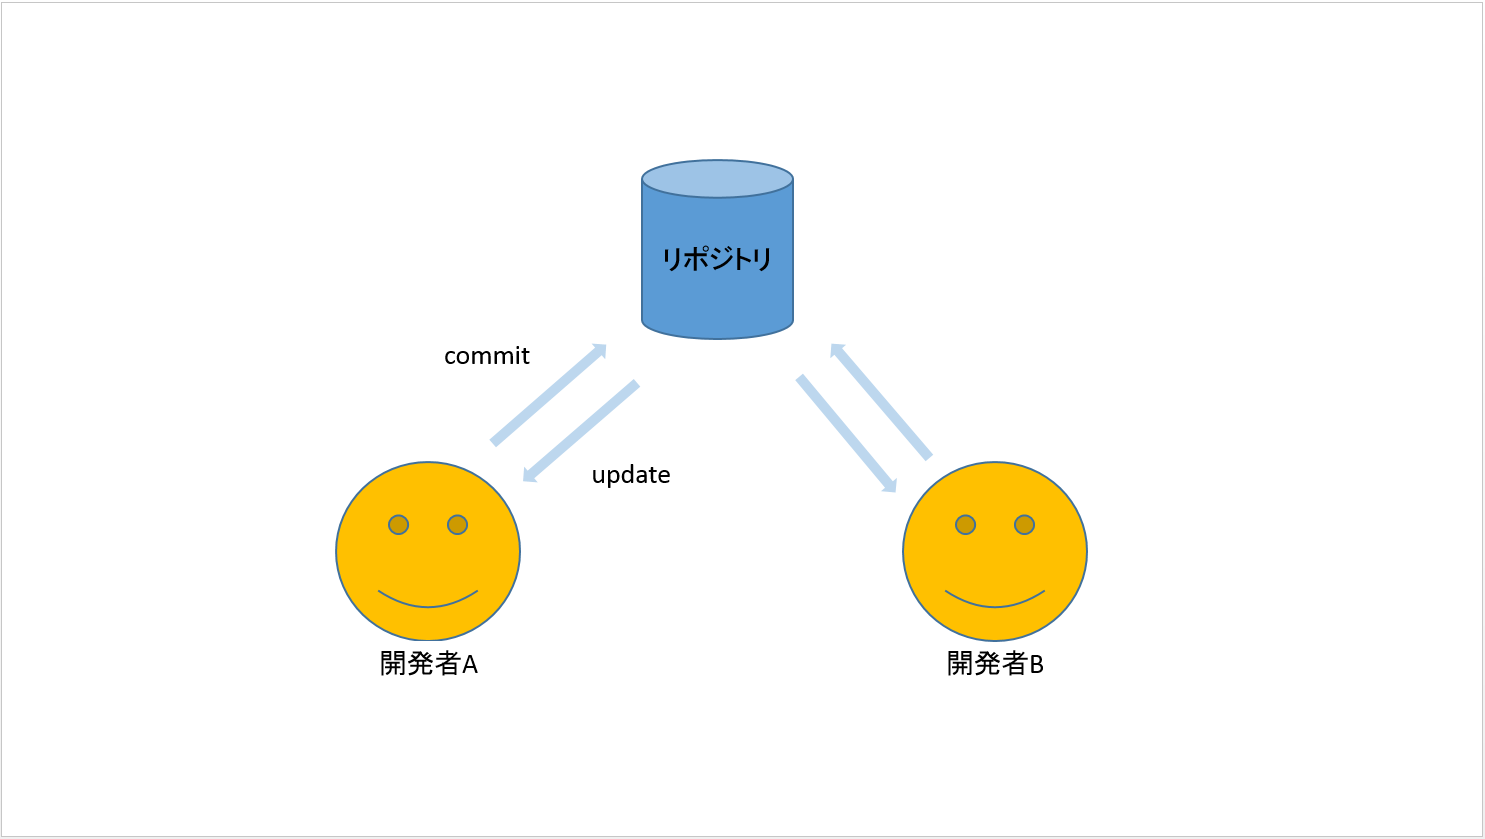
\includegraphics[width=13cm]{syuutyuu.PNG}
\caption{集中型バージョン管理}
\end{figure}

\newpage
分散型は一度サーバからリポジトリを取得しておけばオフラインの状態でも手元の開発環境で編集することができる.分散型は図のように複数リポジトリがあるのが特徴で,手元の開発環境にもリポジトリがあるため,リモートのリポジトリに接続することができない状況でも開発することができるというメリットがある.Gitは分散型バージョン管理システムに区分けされる.

\begin{figure}[htb]
\centering 
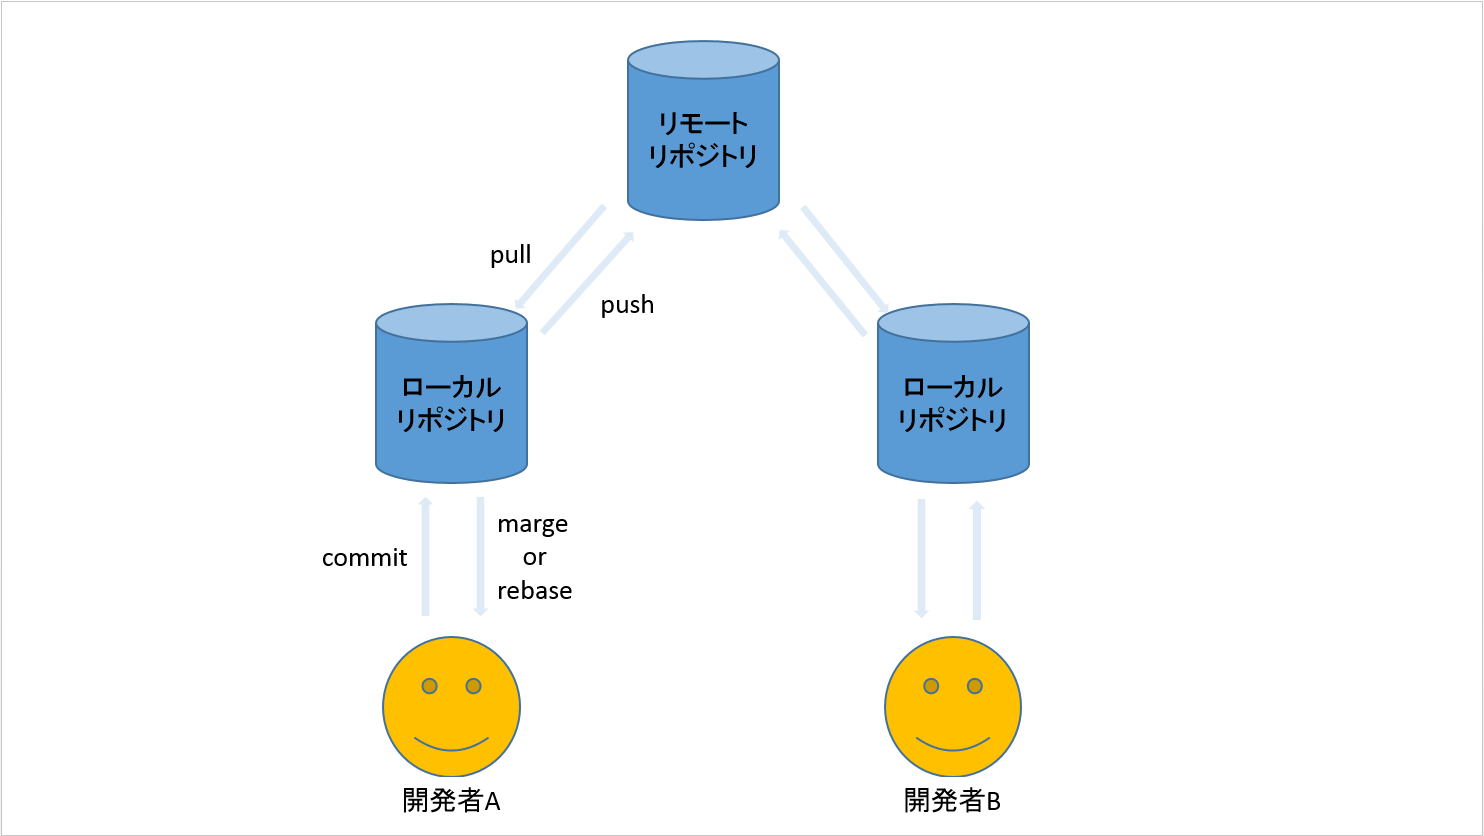
\includegraphics[width=13cm]{bunnsann.PNG}
\caption{分散型バージョン管理}
\end{figure}

\newpage

\section{GitHubとは}
GitHubはGitのリモートリポジトリと様々なWebツールを提供しているサービスである.
リモートリポジトリとはバージョン管理されたファイル群をインターネット上に保管し,それらの取得や変更をすることができる機能のことである.
GitHubで開発を行うことにより地理的に離れたところに住む複数のプログラマによって開発をすることができる.オンラインのコミュニケーションを円滑にするため,GitHubでは相談して課題を解決するIssue(イシュ―),や改善案を手軽に提案できるPull Request(プルリクエスト)などの機能が提供されている.
これらの優れたコラボレーションツールによる開発フローが注目され,オープンソース開発だけでなく,業務での開発にも使われるようになってきました.

\newpage

\section{GitHubのアカウントの取得方法}
\begin{enumerate}
 \item GitHub(https://github.com/)へアクセスする.
 \item ニックネーム,メールアドレス,パスワードを入力して[Sign up for GitHub]をクリックする.なお,パスワードはアルファベット7文字以上で,1文字以上小文字と数字を混ぜる必要があります.
 \item プランを選ぶ.後から変更することができるためここではデフォルトの[Free]プランを選択する.
 \item Continueをクリックするとユーザー登録が完了する.
\end{enumerate}
 
 \begin{figure}[htb]
\centering 
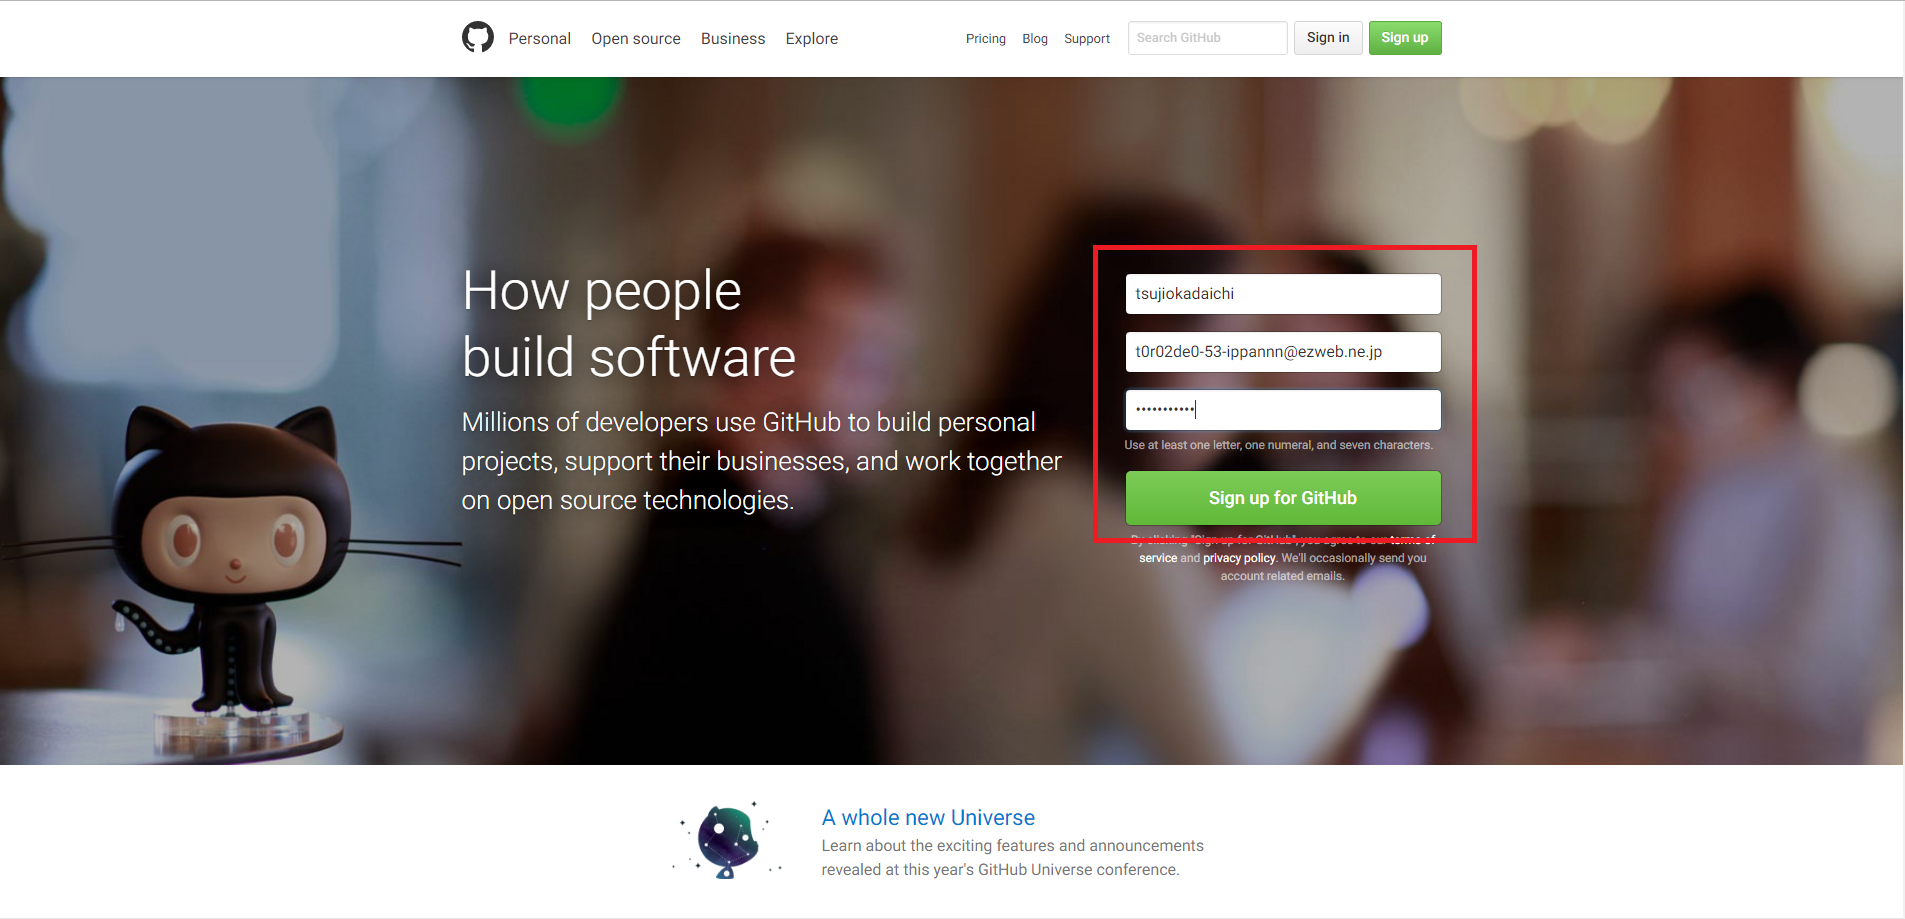
\includegraphics[height=8.5cm,width=13cm]{top.PNG}
\caption{トップページ}
\end{figure}

\newpage



\begin{figure}[htb]
\centering 
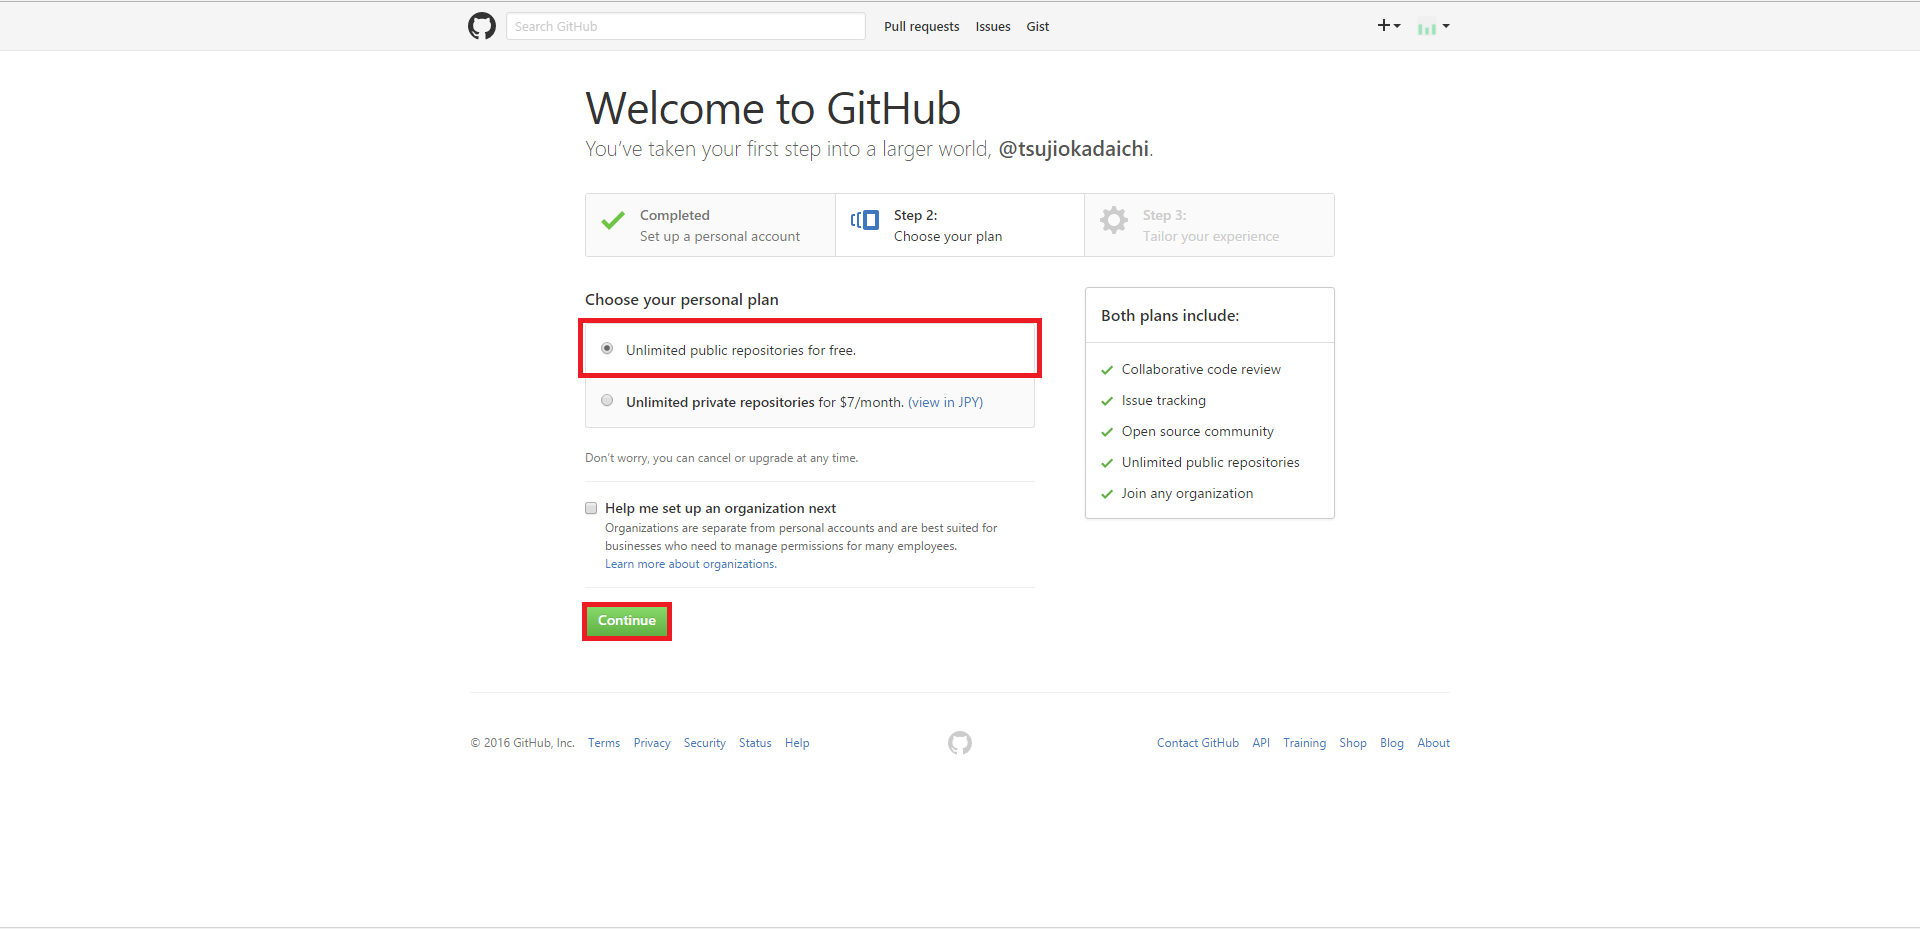
\includegraphics[height=8.5cm,width=13cm]{plan.PNG}
\caption{プランを選んで登録}
\end{figure}

\subsection{メールアドレスを認証する}
ユーザ登録が完了したら,メールアドレスの認証を行た方が良い.不正なサインインに対するセキュリティの強化や,パスワードを忘れた場合にも必要なため,メールアドレスの認証をしておくことをお勧めする.

\newpage
赤い太枠で囲まれているSettingsを選択する.
画面左に表示されているEmailsを選択し,画面右に設置されている「resend」をクリックする.


\begin{figure}[htb]
\centering 
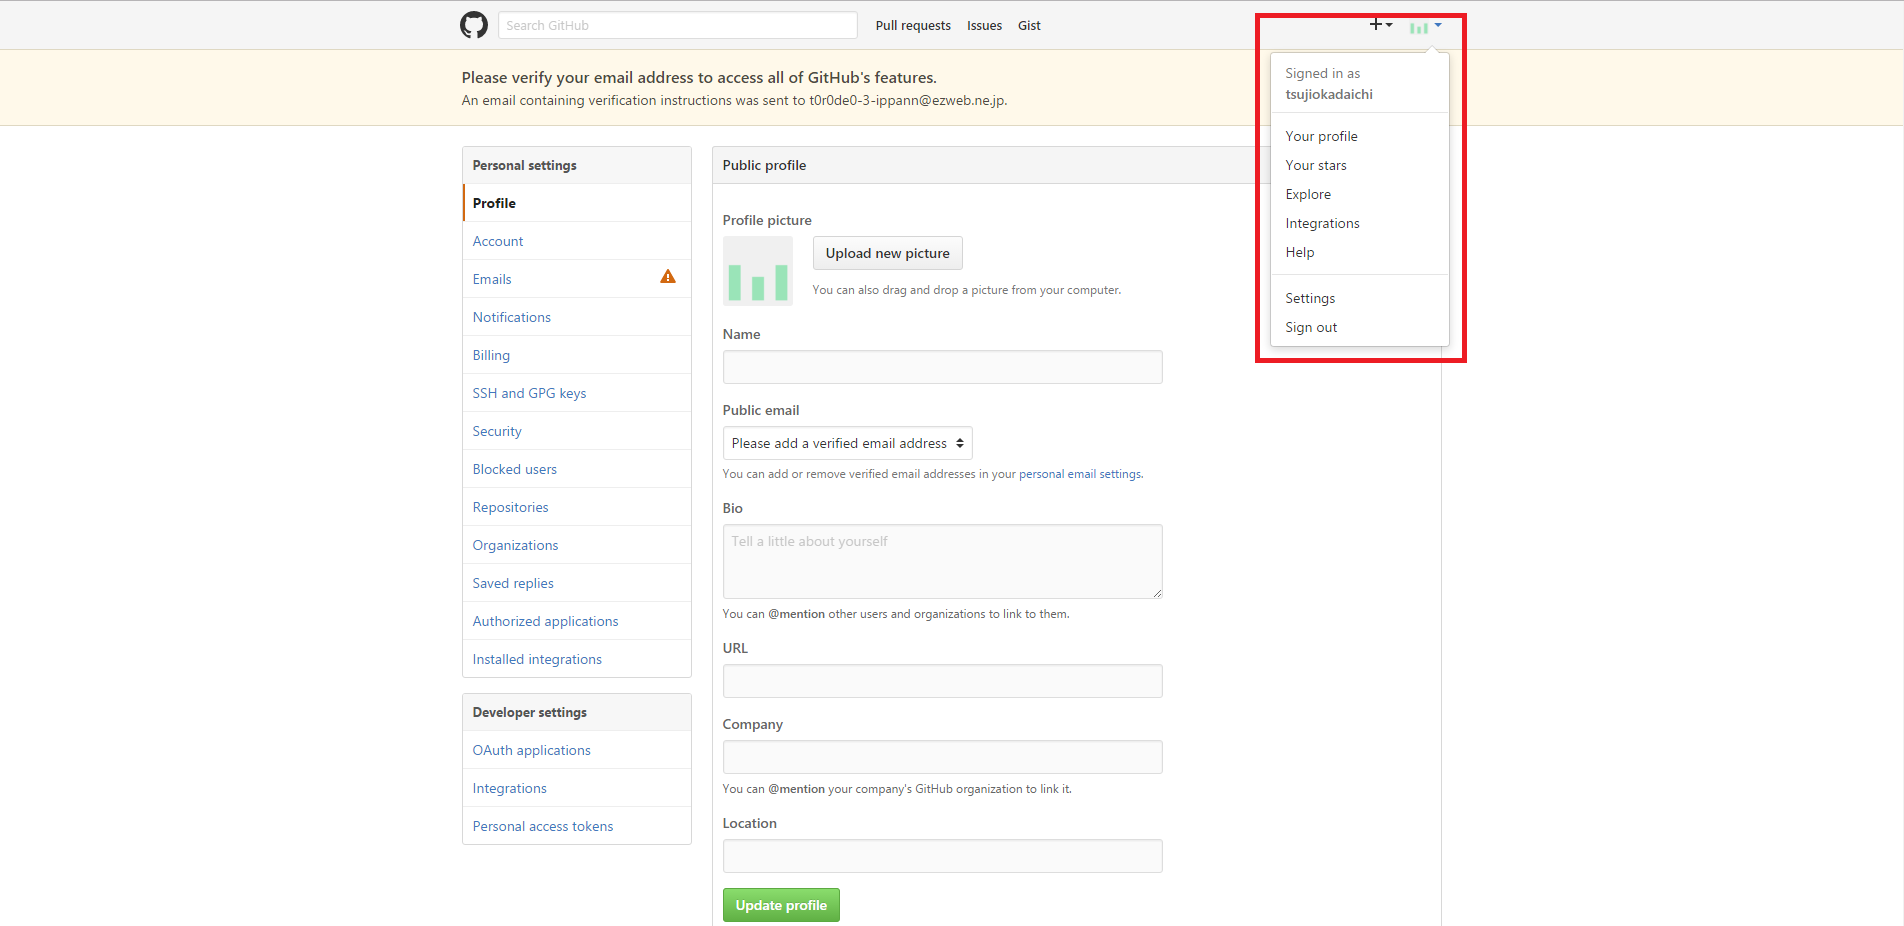
\includegraphics[height=8.5cm,width=13cm]{setting.PNG}
\caption{セッティング}
\end{figure}
 
 
\begin{figure}[htb]
\centering 
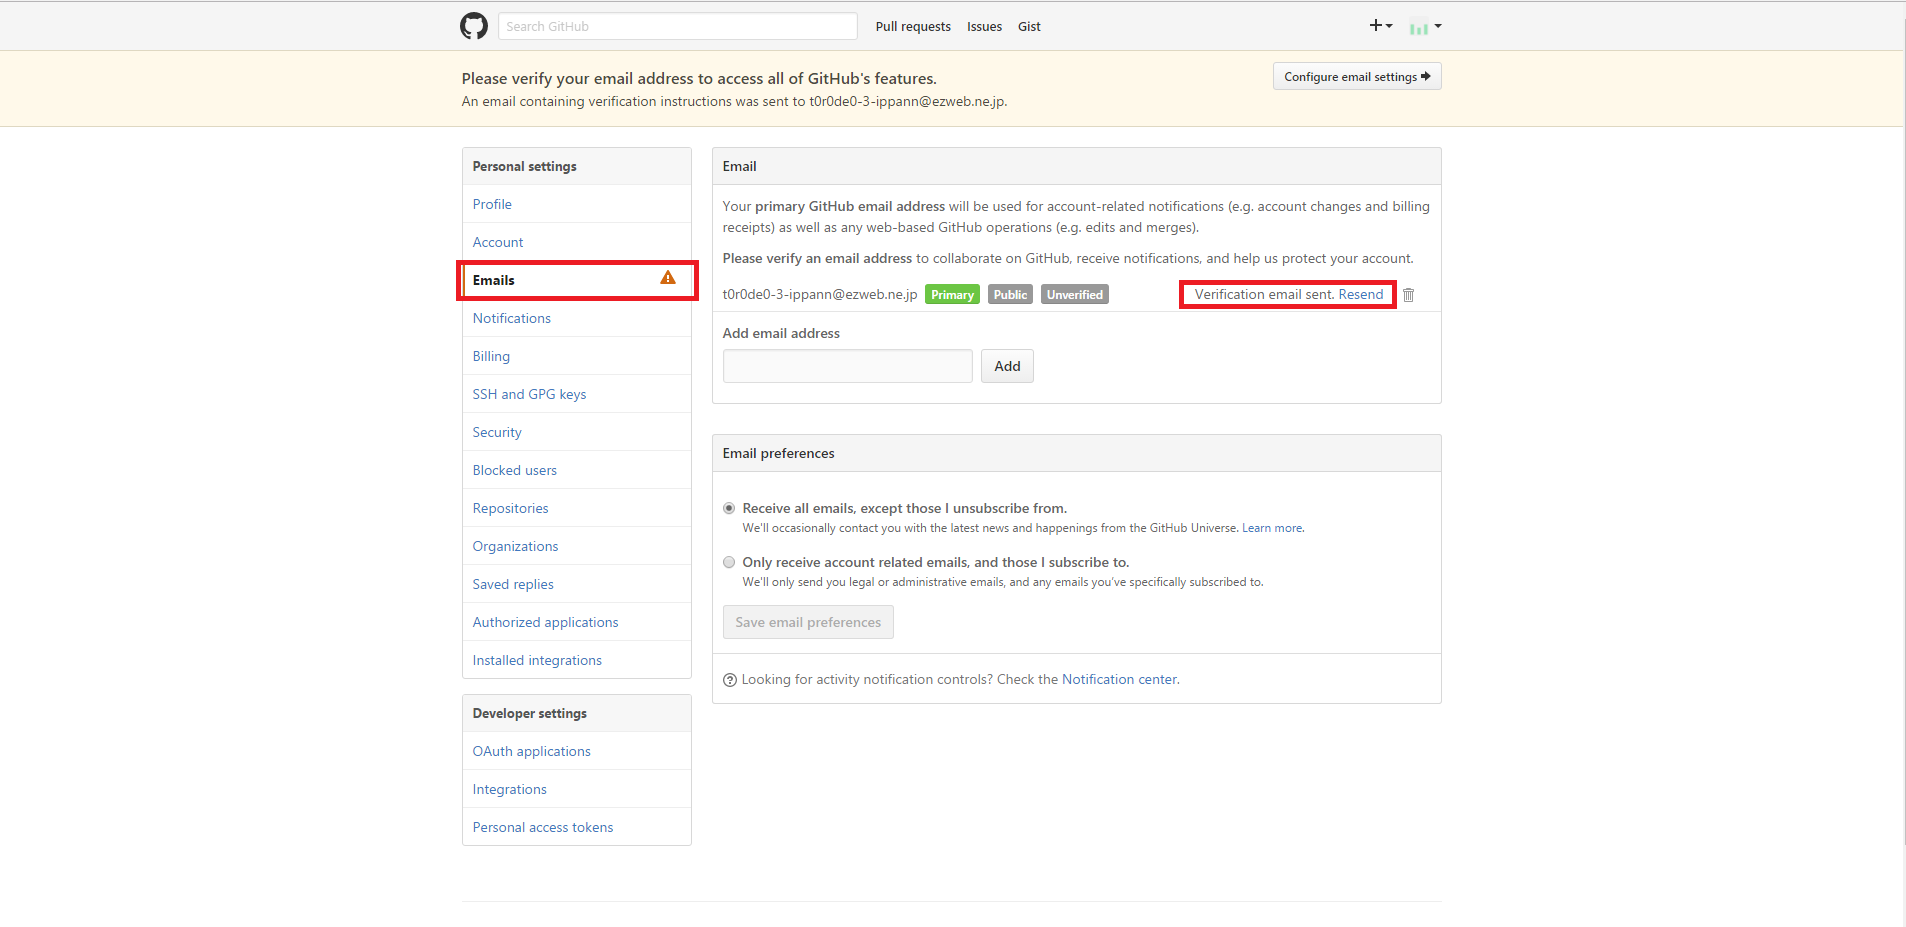
\includegraphics[height=8.5cm,width=13cm]{mail.PNG}
\caption{Emails}
\end{figure}

\newpage
GitHubからメールが届くので,記載されたURLをクリックする.
メール設定画面で該当のメールアドレスが認証済みになったらメールアドレスの認証は完了である.


\begin{figure}[htb]
\centering 
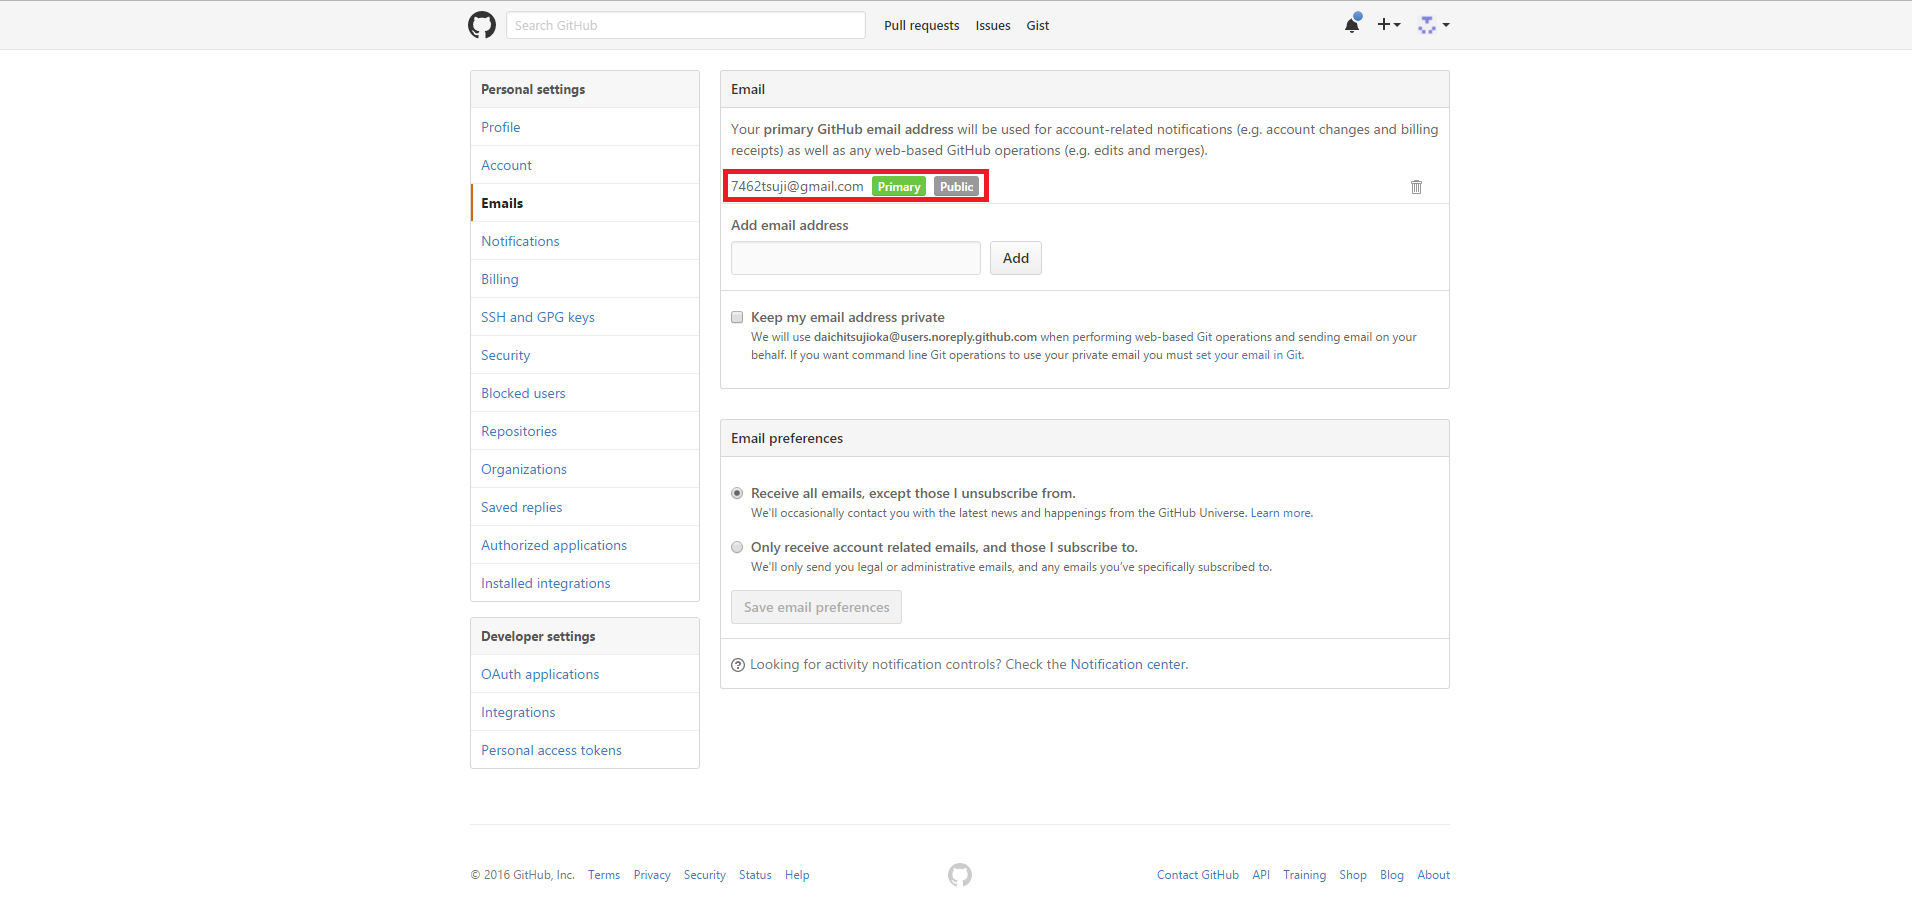
\includegraphics[height=8.5cm,width=13cm]{ok.PNG}
\caption{認証完了}
\end{figure}


\newpage


\section{GitHub用語}

\subsection{リポジトリ}

Gitで管理されたファイルや変更内容が保存される場所.パソコン内にあるものをローカルリポジトリ,GitHubなどローカル以外のサーバ上にあるものをリモートリポジトリと呼ぶ.

\subsection{リモートリポジトリ}

手元に置いてあるローカルなリポジトリ以外の,ネット上に置かれたリポジトリのこと.

\subsection{commit}

変更されたファイルやディレクトリの記録を1まとまりにして,リポジトリに登録(バージョン管理)すること.コミットされた変更内容そのもののことも指す.


\subsection{clone}

ネット上にあるリポジトリをローカルにコピーする機能である.


\subsection{Origin}

clone元のリモートリポジトリのこと.


\subsection{Push}

リモートリポジトリに自分の変更履歴がアップロードされ,リモートリポジトリ内の変更履歴がローカルリポジトリの変更履歴と同じ状態にする機能である.


\subsection{branch}

履歴の流れを分岐して記録していくためのもの.分岐したブランチは,他のブランチの影響を受けないため,同じリポジトリ中で複数の変更を同時に進めていける機能である.


\subsection{pull}

リモートリポジトリから最新の変更履歴をダウンロードしてきて,自分のローカルリポジトリにその内容を取り込む機能である.


\subsection{Pull Request}

相手に対して自分の変更ををpullしてもらうように要求する機能である.


\subsection{Revert}

ステージングエリアに追加した変更を取り消す機能である.

\subsection{タグ}

コミットを参照しやすくするために,わかりやすい名前を付ける機能である.

\subsection{Label}

自由に作成でき,Issueをフィルタリングできる機能である.


\subsection{Merge}

当該ブランチに対して別のブランチの差分を取り込むことである.


\subsection{Fork}

GitHubのサービスで,相手のリポジトリを自分のリポジトリとしてコピー・保持できる機能ある.


\subsection{Issue}

ソフトウェア開発におけるバグや議論などをトラッキングして管理するために発行する.

\subsection{デプロイ}

ソフトウェアの分野で,開発したソフトウェアを利用できるように実際の運用環境に展開する.


\subsection{リリース}

プロセスを次の段階に進めることを認める機能である.


\subsection{Watch}

リポジトリに関する情報をNotificationsに表示する機能である.

\subsection{Star}

リスト一覧からリポジトリを探すことが出来るようにする機能である.
また,注目度を表す指標にもなる.

\subsection{Fork}

GitHub側にある特定のリポジトリを自分のアカウント以下のリポジトリに複製する機能である.

\subsection{人数}

開発人数のことである.
ここでは,Originリポジトリにコミットした人数のことを示す.

\subsection{MileStone}

やるべきタスクの管理にIssueを用いることができるようにする機能である.

\subsection{Wiki}

簡単な記法によってドキュメントを作成,編集するための機能である.

\subsection{マークダウン}

プレーンテキストで手軽に書式を設定して入力できる記法

\subsection{conflict}

複数の人がファイルの同じ場所を変更してしまった場合などに発生し,Gitが自動でマージされできなくなった状態のこと

\subsection{作業ディレクトリ}

リモートリポジトリをcloneしたディレクトリを(ファイル)のことで,バージョン管理されていない(コミットされていない)ファイルも含む

\subsection{ステージングエリア}

ローカルリポジトリ内の領域の1つで,これからコミットするファイルをまとめるために使用する.Source Treeでは「indexにステージしたファイル」と呼ぶ.

\subsection{checkout}

ブランチの切り替えなどによって,作業ディレクトリを指定したコミットの状態にすること.

\subsection{contribution}

ユーザがどの程度GitHub 上で活動しているのかを定量的に知ることができる値である.GitHub上にあるユーザープロフィール画面でグラフと同時に見ることが可能である.\cite{yougo}


\chapter{目的}
GitHubで活発に活動しているユーザはコミュニティが広いのではないかという仮説を検証する.現在システムエンジニアには高いコミュニケーション能力が必要とされている.そこで私は現在システムエンジニアとして活躍している人は高いコミュニケーション能力を備えているのではないかという仮説を立てた.本研究で活発に活動しているユーザのGitHubにおけるcontribution数とGoogle+におけるフォロワー数の相関を取ることができれば,活発に活動しているユーザはコミュニティが広いということが言え,間接的に高いコミュニケーション能力を持っているということが言えるのではないかと考えた.


\chapter{手法}
仮説を検証を行うため以下の方法で研究を進めた.

\begin{enumerate}
 \item GHTorrentから2万件のユーザ情報をランダムサンプリングで抽出した.
 \item 1で抽出したユーザのcontribution数とメールアドレスを,GitHubAPIを用いて取得した.
 \item 取得したメールアドレスを用いGoole+におけるフォロワー数を調べた
 \item ユーザのcontribution数とGoogle+におけるフォロワー数の相関関係を調べた.
\end{enumerate}
GHTorrentとはGitHubのユーザ情報やプロジェクト情報などのすべてのデータが格納されているダンプデータである.また,Google+とはGoogleが運営するSNSのことである.
開発環境としてLinuxを使う.そのためVirtualBoxとubuntuを用意する.

\newpage

\section{Linux}
LinuxとはWindowsやMac OS Xなどと同じオペレーションシステム(OS)である.OSとはPCやスマートフォン,サーバーや組み込み危機を動かすためのソフトウェアである.
Linuxは1991年Linus Torvalds氏によって開発された.その後フリーソフトウェアとして公開され,現在も全世界の有志の開発者によって改良が重ねられている.
Linuxの特徴として
\begin{enumerate}
 \item 無料である
 \item オープンソフトウェアである
 \item 性能が低いPCでも動作可能である
 \item 多くの企業,組織で採用されている
 \item 様々なディストリビューションがある.例えばUbuntuやCentOSなどがある.
\end{enumerate}
などが挙げられる.

\newpage

\section{Chocolatey}
VirtualBoxをインストールするにあたり,まずはChocolateyをインストールする.Chocolateyをインストールせずとも作業を進めることは可能だが,Chocolateyをインストールすることにより開発環境を簡単に整えることができるためである.
ChocolateyとはWindows上で動作するソフトウェアをコマンドラインからインストール,アンインストール,アップデート,検索することができるパッケージマネージャーである.
Windows上で開発環境を整えるためには
\begin{enumerate}
 \item 使用したいツールの公式サイトにアクセスする.
 \item インストーラーを探してダウンロードする.
 \item インストーラーを実行する.
\end{enumerate}
という手間がかかってしまう.

\newpage
しかしChocolateyをインストールすることにより,管理者権限のあるコマンドプロンプトに


\begin{figure}[htb]
\centering
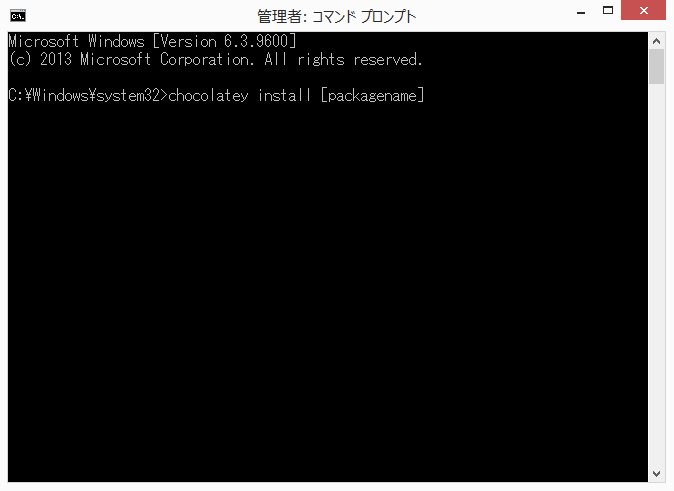
\includegraphics[width=12cm]{choco.PNG}
\caption{Chocolateyの使用例}\label{サンプル図}
\end{figure}


上の画像のようなコマンドを打ち込むだけでインストールができるようになる.Chocorateyをインストールすることによるメリットとして
\begin{itemize}
 \item 使いたいソフトのWindowsインストーラをダウンロードする手間が省ける.
 \item Chocolateyでインストールしたソフトは一括でアップデートできる.
 \item 広告URLをクリックしてしまい間違ったソフトをうっかりダウンロードしてしまう心配がなくなる
\end{itemize}
などのメリットが挙げられる.

\newpage

\subsection{Chocolateyのインストール}
管理者権限のあるコマンドプロンプトを開く.Chocolateyのサイトに掲載されているコマンドを実行する.

\begin{figure}[htb]
\centering
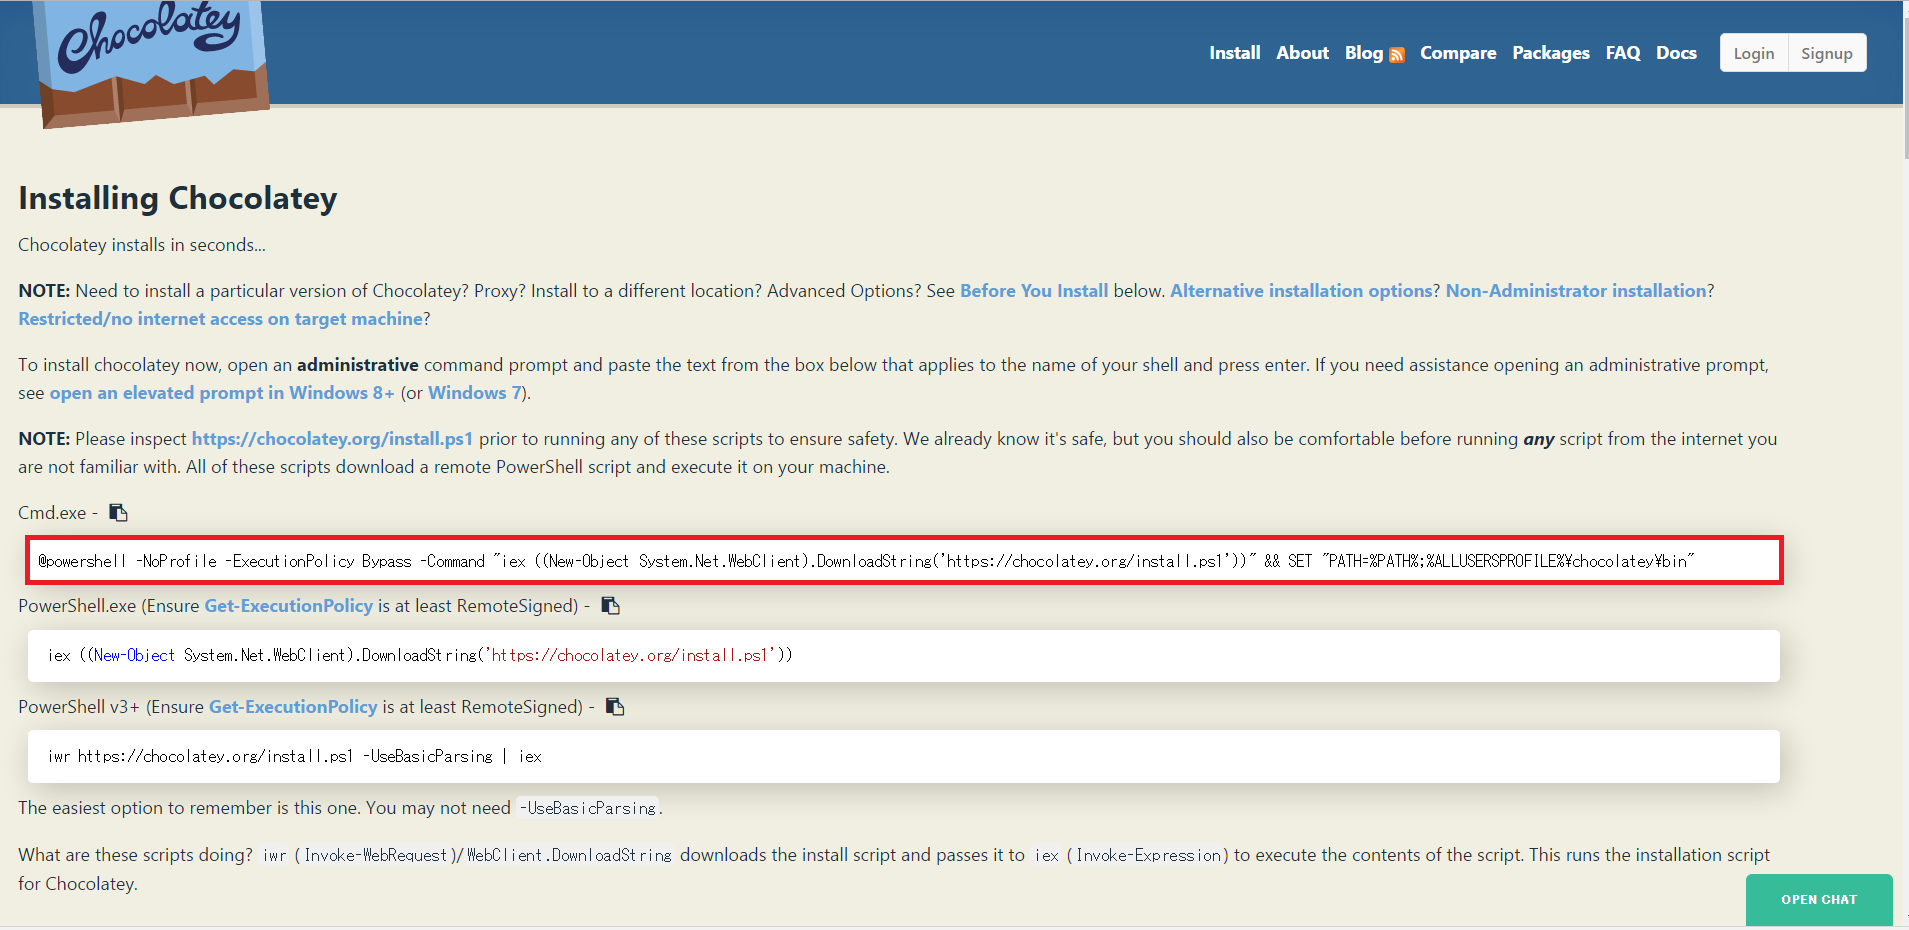
\includegraphics[height=8.5cm,width=10cm]{chocohomepage.PNG}
\caption{Chocorateyのインストールコマンド}\label{サンプル図}
\end{figure}
上の画像の赤枠で囲んであるコマンドをコピーし貼り付けEnterキーを押すことでChocolateyをインストールすることができる.

\newpage

\section{VirtualBox}
本研究では,LinuxOSを扱いたいが,パソコン本体はWindowsOSの為,このソフトを利用する.VirtualBoxとは,使用しているパソコン上に仮想的なパソコンを作成し,別のOSをインストール・実行できるフリーのパソコン仮想化ソフトのことである.

%図の挿入
\begin{figure}[htb]
\centering
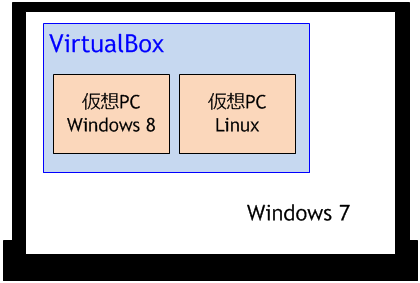
\includegraphics[width=12cm]{virtualbox.png}
\caption{VirtualBoxのイメージ}\label{サンプル図}
\end{figure}
VirtualBoxはコンピュータ上で直接動作している通常のOSにとってはアプリケーションの一つであり,ほかのソフトと同じように起動することができる.起動すると仮想的なコンピュータが構築され,元のOSとは独立に別のOSを起動することができる.VirtualBoxが実行されているOSをホストOS,VirtualBox上で実行されているOSをゲストOSという.
元は独立系のソフトウェア企業が開発・販売していた製品だった.しかし,開発元がSun Microsystems社に買収され,その後同社がOracle社に買収されたため,Oracle社が開発元となり,正式名称も「Oracle VM VirtualBox」となった.また,VirtualBox本体はGPLに基づいたオープンソースソフトウェアとして公開され,だれでも自由に入手・利用・改変・再配布などが行える.
VirtualBoxを使う上での注意点
現時点でのVirtualBoxは仮想メモリをサポートしていないため,実メモリ以上のメモリを仮想PCが使用することはできない.仮想メモリを使うと動作が遅くなるため,仮想PCには実メモリ以内のサイズを割り当てる.そのため,仮想PCを1台だけ起動するのであれば問題ないが,複数の仮想PCを同時に起動させる場合これがネックになってしまう.同時起動させる全ての仮想PCのメモリサイズの合計が実メモリのサイズを超えないようにする.そのため,VurtualBoxをインストールするPCには多くのメモリが必要で,最低4GB以上のPCを使うようにするべきである.

\newpage

\subsection{VirtualBoxのインストール}
Chocolateyをインストールした後,管理者権限のあるコマンドプロンプトでVirtualBoxのダウンロードサイトに掲載されているコマンドを実行する.

%図の挿入
\begin{figure}[htb]
\centering
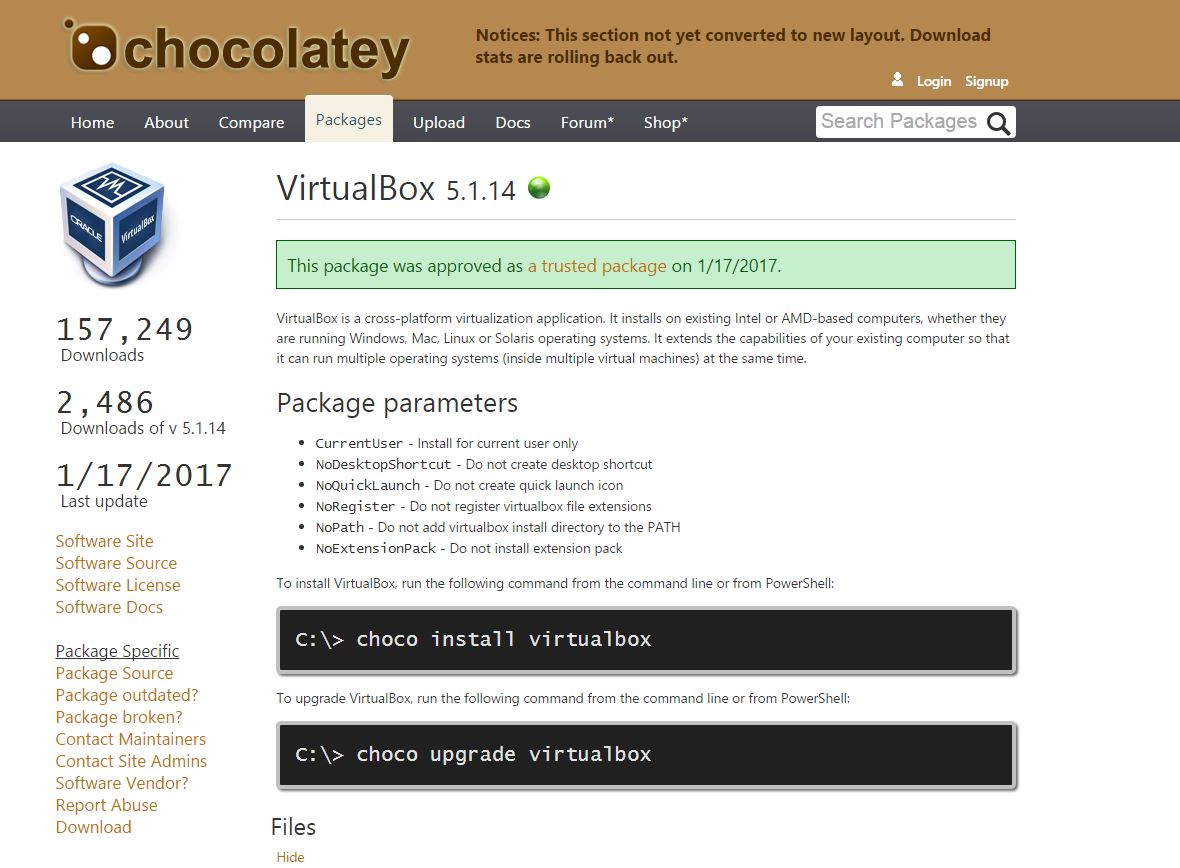
\includegraphics[width=12cm]{VirtualBox.JPG}
\caption{VirtualBoxのインストール}\label{サンプル図}
\end{figure}


ダウンロードサイト

https://chocolatey.org/packages/virtualbox

\newpage

%図の挿入
\begin{figure}[htb]
\centering
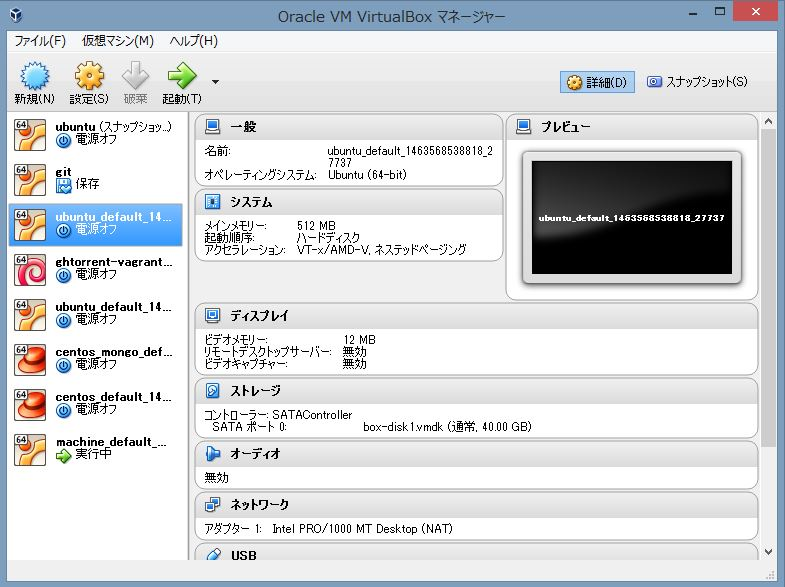
\includegraphics[width=12cm]{virtualboxkidou.JPG}
\caption{VirtualBox.exe起動画面}\label{サンプル図}
\end{figure}


インストールした「VirtualBox.exe」を起動して正常に動作するか確認する.

\newpage

\subsection{VirtualBoxの用語}

\subsubsection{ホストマシン}

物理的に存在するコンピュータのこと.

\subsubsection{ホストOS}

ホストマシンにインストールされているOSのこと.VirtualBoxはホストOSにインストールされる.

\subsubsection{バーチャルマシン(仮想マシン)}

VirtualBoxが作成する論理的なマシンのこと.ゲストマシンに割り当てるために,VirtualBoxがホストマシンのコンピュータ資源(CPUやメモリ,HDD等)の一部を仮想化する.ホストマシンの資源を使い切らない限り,ゲストマシンを複数作成したり,多重起動させることができる.

\subsubsection{ゲストOS(仮想OS)}

ゲストマシンにインストールされるOSのこと.

\subsubsection{仮想ディスク}

ゲストマシンが使用する仮想のハードディスクのこと.バーチャルマシンからはこれを物理ディスクとして扱うことができる.仮想ディスクの実態はホストマシン内にファイルとして存在する.

\newpage

\section{Tera Term}

Teratermとはネットワークを経由してほかのコンピュータに接続し,遠隔操作をするための仕組みである.
Chocolateyをインストールした後,管理者権限のあるコマンドプロンプトでTeraTermのダウンロードサイトに掲載されているコマンドを実行する.

%図の挿入
\begin{figure}[htb]
\centering
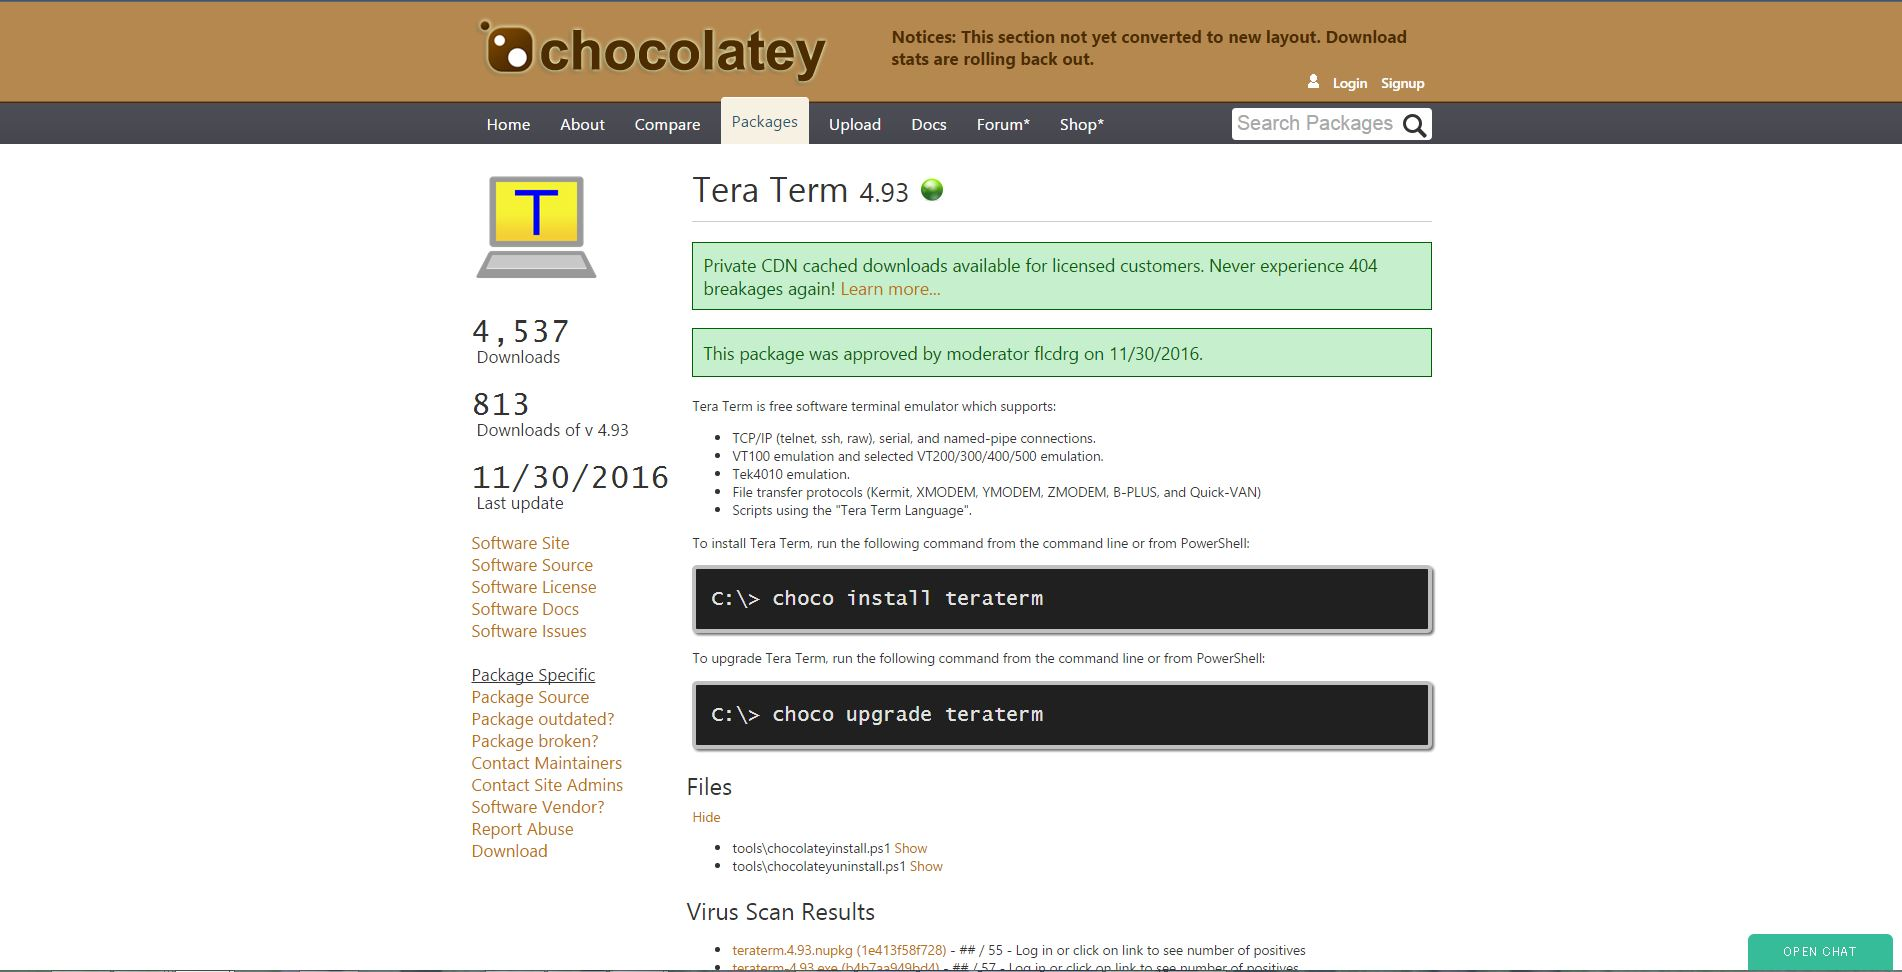
\includegraphics[width=12cm]{teraterm.JPG}
\caption{TeraTermのインストール}\label{サンプル図}
\end{figure}

ダウンロードサイト

https://chocolatey.org/packages/teraterm/

%図の挿入
\begin{figure}[htb]
\centering
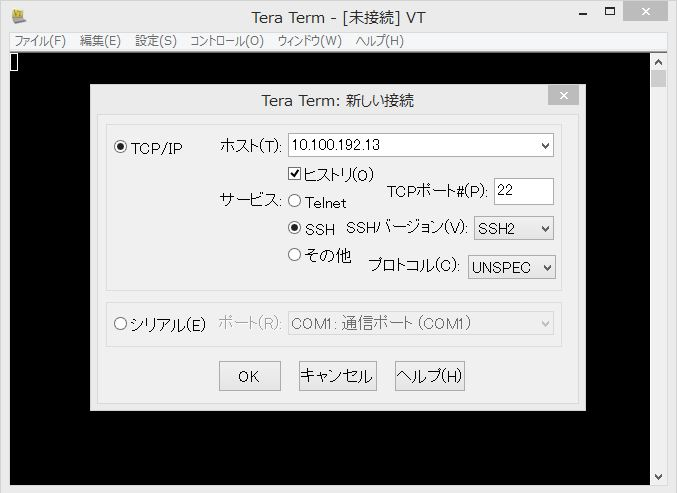
\includegraphics[width=12cm]{teraterm2.JPG}
\caption{TeraTerm起動画面}\label{サンプル図}
\end{figure}

\newpage

\section{MySQL}
GHTorrentのデータを扱うためには用意した仮想環境にMySQLを導入する必要がある.

\subsection{MySQLとは}
MySQLとはオープンソースのリレーショナルデータベース管理システム(RDBMS)である.処理速度を最重要視して開発が進められたため,処理速度は商用データベースにも劣らない.オープンソース系としては世界的に最も多く導入されており,FacebookやTwitter,Amazonなど有名企業も導入している.
MySQLは無料で使うことができるが,さまざまな機能が実装されているので,使いこなすためにはかなりの経験が必要になる.
MySQLをどのようにデータを管理しているかを簡単に書くと以下の画像のようになる.NySQLは一つ以上のデータベースを持ち,各データベースまたは一つ以上のテーブルを持つ.\cite{mysql}

\begin{figure}[htb]
\centering 
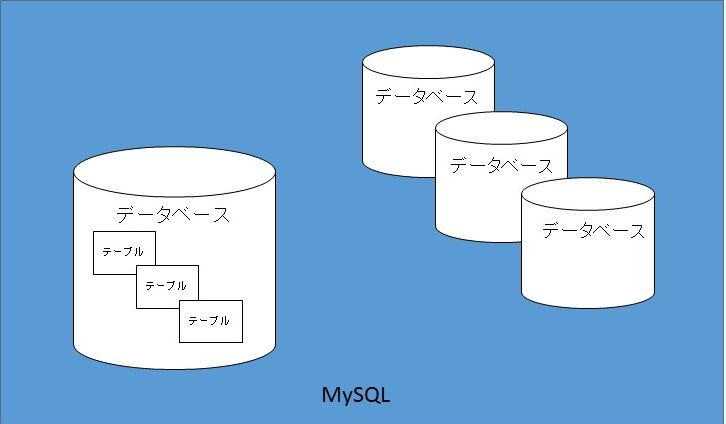
\includegraphics[height=8.5cm,width=13cm]{mysqltoha.JPG}
\caption{MySQLのイメージ}
\end{figure}


\subsection{MySQLのインストール}
yumコマンドを利用してMySQLサーバのインストールを行う.以下のコマンドを入力し,実行することでインストールが開始される.

yum -y install mysql-server

\newpage

\subsection{MySQLのコマンド}

\subsubsection{mysql -u (ユーザ名)}
起動するためのコマンド

\subsubsection{mysql -u(ユーザ名) -p}
パスワードを入力して起動するコマンド

\subsubsection{create database (データベース名) default character set utf8}
データベースを作成するためのコマンド

\subsubsection{drop database (データベース名)}
データベースを削除するためのコマンド

\subsubsection{use (データベース名)}
データベースを起動するためのコマンド

\subsubsection{select * from (テーブル名)}
データの中身を確認するためのコマンド

\subsubsection{select (取り出したいデータ) from (対象のテーブル) where (対象を限定する条件)}
データベースから特定のデータを検索するためのコマンド

\subsubsection{create database (データベース名)}
データベースを作るためのコマンド

\subsubsection{show databases}
データベースの中身を確認するためのコマンド

\subsubsection{show tables}
データベース内に存在するテーブルの確認するためのコマンド



\newpage

\section{GHTorrent}
ここではGHTorrentのデータをMySQLにインポートして利用する方法を解説する.
前提知識として
\begin{itemize}
\item 「Webアプリケーション構築入門」の第7章を読みMySQLについて学習する.
\item テーブルの構成を,「http://gousios.gr/bibliography/GS12.html」に掲載されている図で確認する.
\end{itemize}
 以上の2点を行っておいたほうが良い.
 
 \subsection{MySQLへのインポート}
  GHTorrentのMySQL用データをダウンロードし,共有フォルダに置いておく.
 コマンドラインでパスワードを書いたときに警告が出てしまうため,MySQLのパスワードを環境変数に入れておく.
 
\begin{lstlisting}[basicstyle=\ttfamily\footnotesize, frame=single]
export MYSQL_PWD=pass
export dbname=ghtorrent20161101
\end{lstlisting}
 
 /etc/mysql/mysql.cnfに以下を追記し,sudo service mysql restart.なお主記憶16G程度のマシンを想定している.メモリが少ない場合はそれに応じて数値を減らす必要がある.
 
\begin{lstlisting}[basicstyle=\ttfamily\footnotesize, frame=single]
[mysqld]
skip-external-locking
key_buffer_size = 4096M
max_allowed_packet = 1M
table_open_cache = 512
sort_buffer_size = 2M
read_buffer_size = 2M
read_rnd_buffer_size = 8M
myisam_sort_buffer_size = 4096M
thread_cache_size = 8
query_cache_size = 32M
\end{lstlisting}
 
共有フォルダをマウントする.
 
\begin{lstlisting}[basicstyle=\ttfamily\footnotesize, frame=single]
cd
mkdir share
sudo mount -t cifs //10.100.192.3/share share -o user=guest
\end{lstlisting}
 ダウンロード積みのファイルをMySQLがアクセスできる場所で展開する.
 
\begin{lstlisting}[basicstyle=\ttfamily\footnotesize, frame=single]
cd /tmp
tar xf ~/share/ghtorrent/mysql-2016-11-01.tar.gz
\end{lstlisting}

\newpage
schema.sqlを修正し,インデックスをすべて削除する.

\begin{lstlisting}[basicstyle=\ttfamily\footnotesize, frame=single]
cp schema.sql schema.sql.bak

grep CONSTRAINT schema.sql | \
gawk '{print "ALTER TABLE",$2,"DROP FOREIGN KEY",$2,";"; print
 "ALTER TABLE",$2,"DROP INDEX",$2,";";}' | \
sed 's/_ibfk_.//' | \
sed 's/_fk./s/' \
>> schema.sql
\end{lstlisting}
ght-restoreを修正する.

\begin{itemize}
\item LOAD DATAのファイルの場所を自由にする..
\item SQLの宣言を緩和する.
\item 「\#3」以降,つまりインデックスの作成を止める.
\end{itemize}
修正点は以上の3つである.

\begin{lstlisting}[basicstyle=\ttfamily\footnotesize, frame=single]
cat ght-restore-mysql | \
sed "s/; LOAD DATA INFILE/, SQL_MODE='TRADITIONAL,ALLOW_INVALID_DATES';
 LOAD DATA LOCAL INFILE/" | \
sed 's/$mysql/$mysql --local-infile --force/g' | \
gawk '{ if($0!~/# 3/) print $0; else exit 0; }' \
> ght-restore-mysql2
\end{lstlisting}
データベースを作成する.
\begin{lstlisting}[basicstyle=\ttfamily\footnotesize, frame=single]
echo "drop database if exists $dbname; create database $dbname;" | mysql -uroot
\end{lstlisting}

\newpage

\subsection{データの確認}
インポートが完了したかを確認する.まずはMySQLを起動する.
以下のコマンドで起動することができる.
\begin{lstlisting}[basicstyle=\ttfamily\footnotesize, frame=single]
mysql -uroot -pass
\end{lstlisting}
 
 %図の挿入
\begin{figure}[htb]
\centering
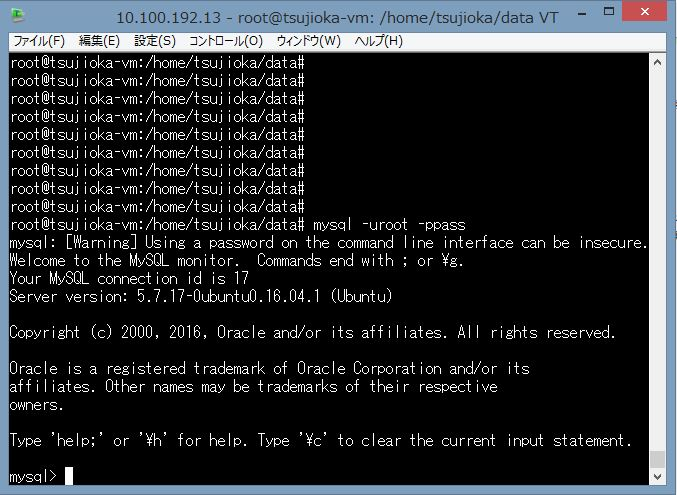
\includegraphics[width=12cm]{mysql.JPG}
\caption{MySQL起動画面}\label{サンプル図}
\end{figure}
上の画像のようになったらMySQLを起動することができた.
 

\newpage
データベース一覧を表示することにより,GHTorrentのダンプファイルがMySQLに入っていることを確認する.
以下のコマンドでデータベース一覧を表示させる.
\begin{lstlisting}[basicstyle=\ttfamily\footnotesize, frame=single]
show databases;
\end{lstlisting}
 
\begin{figure}[htb]
\centering
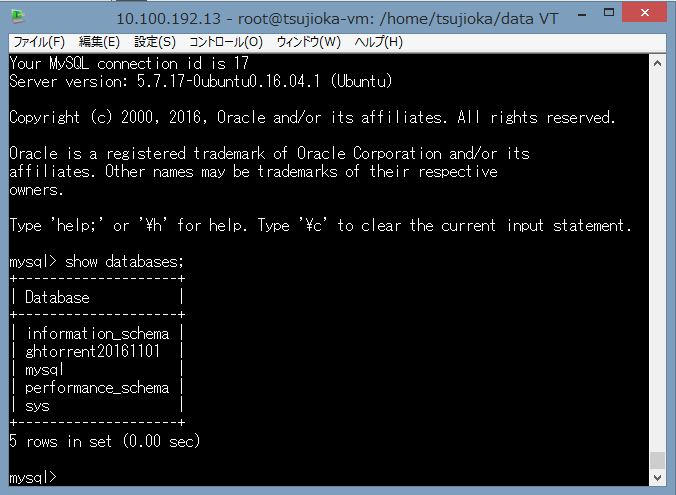
\includegraphics[width=12cm]{showdatabase.JPG}
\caption{データベース一覧}\label{サンプル図}
\end{figure}
 
\newpage
GHTorrentのダンプファイルがMySQLに入っていることを確認した後,ユーザのデータを作業フォルダに移すためデータベースを選択する.
以下のコマンドでデータベースを選択する.
\begin{lstlisting}[basicstyle=\ttfamily\footnotesize, frame=single]
use ghtorrent20161101;
\end{lstlisting}
Detabase changedと表示されたらデータベースを選択することができた.
ghtorrent20161101の構成は下の画像のようになっている.
\begin{figure}[htb]
\centering
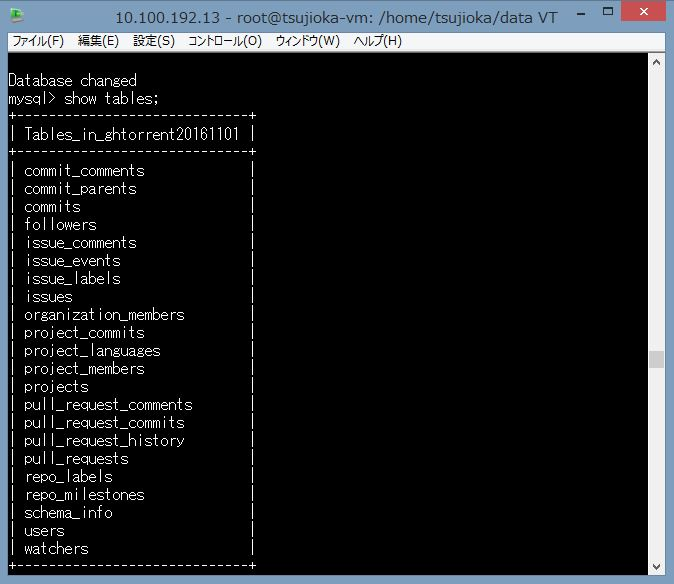
\includegraphics[width=12cm]{showtables.JPG}
\caption{テーブル一覧}\label{サンプル図}
\end{figure}

usersというテーブルに本研究で用いるGitHubの全ユーザ情報が格納されている.


\newpage

usersというテーブルの仕様を確認する.
以下のコマンドで確認できる.
\begin{lstlisting}[basicstyle=\ttfamily\footnotesize, frame=single]
desc users;
\end{lstlisting}

\begin{figure}[htb]
\centering
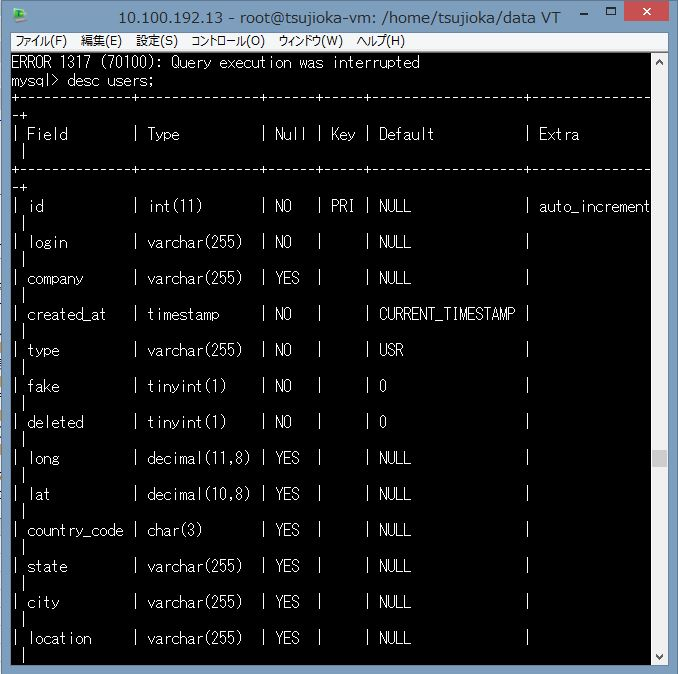
\includegraphics[width=12cm]{descusers.JPG}
\caption{テーブルの仕様}\label{サンプル図}
\end{figure}
usersというテーブルは上の画像のような仕様となっている.
このテーブル内にあるloginというカラムにユーザ名が格納されている.

\newpage

試しに私のユーザ情報を検索してみる.
以下のコマンドで検索できる.
\begin{lstlisting}[basicstyle=\ttfamily\footnotesize, frame=single]
select * from users where login='daichitsujioka';
\end{lstlisting}

\begin{figure}[htb]
\centering
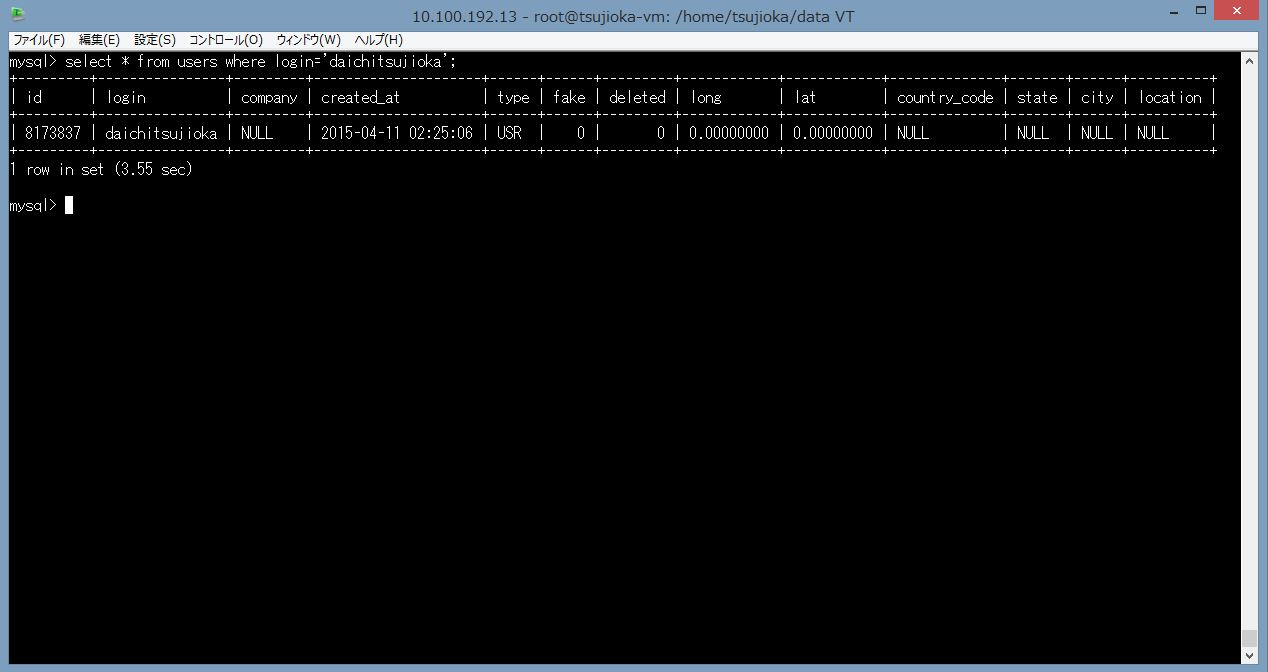
\includegraphics[height=8.5cm,width=13cm]{example.JPG}
\caption{検索例}\label{サンプル図}
\end{figure}
上の画像がGHTorrentに格納されている私のユーザ情報である.


 \section{エクスポート}
 
GHTorrentのダンプファイルがMySQLに格納されていることを確認することができたら,APIを使うことができる仮想環境に移動する.
以下のコマンドでMySQLに格納されているユーザ名だけを仮想環境に移動することができる.
\begin{lstlisting}[basicstyle=\ttfamily\footnotesize, frame=single]
select login form users into outfile `/var/lib/mysql-files/user.txt';
\end{lstlisting}

\newpage

エクスポートしたデータを作業フォルダに移動するために以下のコマンドを使用する.
\begin{lstlisting}[basicstyle=\ttfamily\footnotesize, frame=single]
mv user.txt \home\tsujioka\data;
\end{lstlisting}

作業フォルダにuser.txtが移動できたか確認する.

\begin{figure}[htb]
\centering
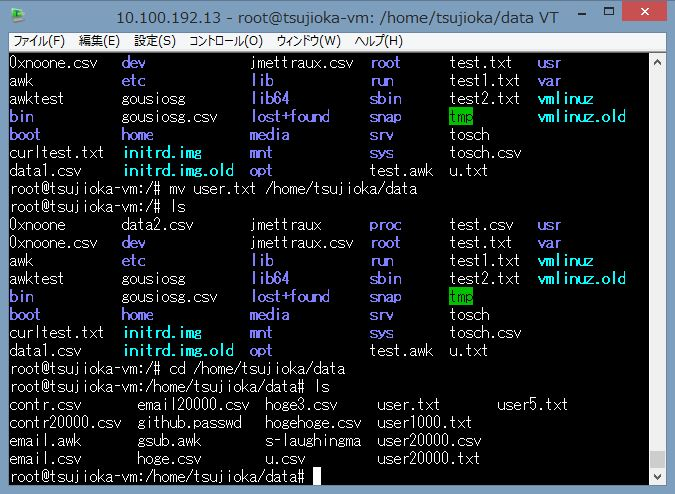
\includegraphics[width=12cm]{kakuninn.JPG}
\caption{データの移動}\label{サンプル図}
\end{figure}


\newpage


\section{ランダムサンプリング}

ユーザ情報をデータベースから作業フォルダへ移すことができた後,ランダムサンプリングを行い,全ユーザから20000人分のデータを取得した.

\begin{itemize}
 \item APIを用いて全ユーザの情報を集めると膨大な時間がかかってしまうため.
 \item 全ユーザの情報を集めることはできないが,推測統計学の数学的研究から,全体のごく一部を調べるだけで,大きな母集団の正確な情報をつかめるということが実験的にも理論的にも証明されているため
 \end{itemize}

以上2点の理由からランダムサンプリングを行って研究を進めた.

以下が全ユーザ情報が入っているuser.txtから20000人分のユーザ情報をランダムサンプリングするためのコマンドである.

\par

\begin{lstlisting}[basicstyle=\ttfamily\footnotesize, frame=single]
shuf -n 20000 /user.txt > user20000.csv
\end{lstlisting}

%図の挿入
\begin{figure}[htb]
\centering
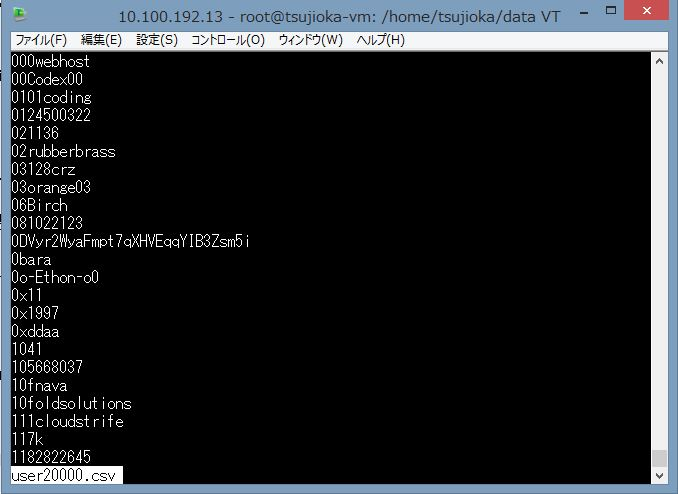
\includegraphics[width=12cm]{rand.JPG}
\caption{ランダムサンプリング}\label{サンプル図}
\end{figure}

\newpage


 
 \section{GitHubAPI}
GitHubAPIを使用することによりGitHub上でいろいろな操作をすることが可能になる.
APIとはアプリケーションプログラムインターフェースの略称で,プログラミングの際に使用できる命令や規約,関数などの集合のことを指している.ソフトウェア開発の際,いちからすべてを作るよりAPIを利用すればもともとあるプログラムを呼び出して,その機能を組み込んだソフトウェアを開発することができる.
システム開発をする際にプログラムをパーツ化して再利用できるようにするSOA(サービス指向アーキテクチャ)も似たような考えだが,システム内での利用にとどまらず,外部ネットワークからモバイル端末を通して,システム機能を呼び出して利用する仕組みとしてAPIは適している.
現在Webサービスの提供事業者は自社サービスを普及させるために自社サービスの機能の一部などを積極的に公開している.この時に利用される仕組みもAPIである.逆に幅広く普及しているサービスと自社のアプリケーションやWebサービスをAPIで連携させることにより自社サービスの価値を向上させることもできる.また,APIを公開して,機能の利用に応じて課金するビジネスモデルも一般的になっている.

GitHubAPIを使用することによりできることの例
\begin{itemize}
 \item NotificationsやFeedsの取得
 \item Gistの生成・更新・取得・削除
 \item Issuesの生成・更新・取得・削除
 \item Organizationsの一覧やメンバーの取得
 \item Repositoryの生成・更新・取得・削除
\end{itemize}
などを行うことができる.

\newpage


\subsection{メールアドレス}
20000人分のユーザ情報を取得することができた後,Emailアドレスを取得するためのAPIを実行する.
以下がEmailアドレスを取得するためのAPIである.


\begin{lstlisting}[basicstyle=\ttfamily\footnotesize, frame=single]
for i in `cat user20000.csv`;do
curl -s -u $(cat github.passwd) "https://api.github.com/users/$i" 
| grep email | gawk -v i=$i -f email.awk >> email20000.csv
echo $i
done
\end{lstlisting}



%図の挿入
\begin{figure}[htb]
\centering
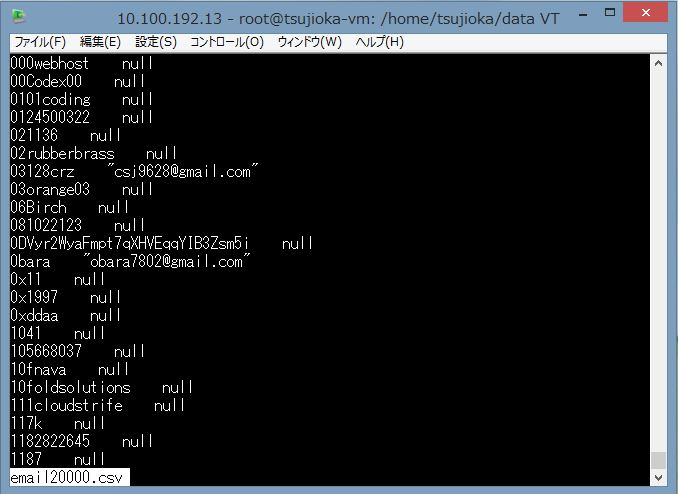
\includegraphics[width=12cm]{email20000.JPG}
\caption{メールアドレス取得}\label{サンプル図}
\end{figure}
上の画像のようなデータを取得することができたら成功である.
なお,メールアドレスがnullになっているユーザはメールアドレスを登録していないユーザである.

\newpage

\subsection{contribution}
GitHubAPIによりEmailアドレスを取得することができた後,contributionを取得するためのAPIを実行する.
以下がcontributionを取得するためのAPIである.

\begin{lstlisting}[basicstyle=\ttfamily\footnotesize, frame=single]
for i in `cat user20000.csv`;do
curl -s -u $(cat github.passwd) "https://github.com/users/$i/contributions" 
| grep -o data-count=.*d | gawk -v i=$i -f gsub.awk >> contr20000.csv
echo $i
done
\end{lstlisting}



%図の挿入
\begin{figure}[htb]
\centering
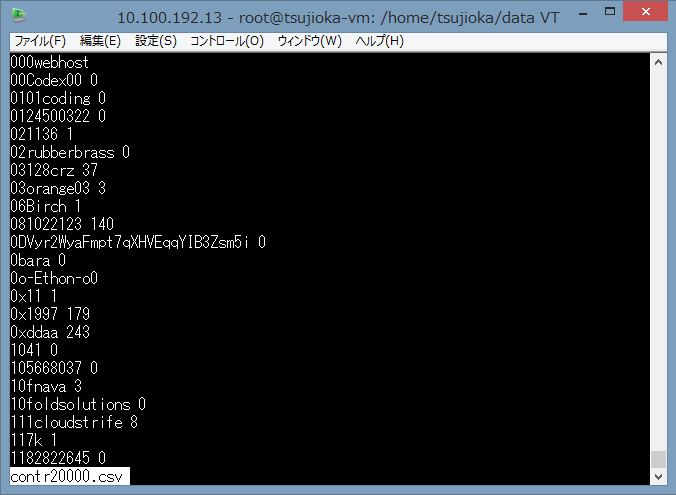
\includegraphics[width=12cm]{contr20000.JPG}
\caption{contribution取得}\label{サンプル図}
\end{figure}
上の画像のようなデータを取得することができたら成功である.
なお,contribution数が入るべき場所が空白になっているユーザはすでにGitHubを退会してしまっているユーザである.

\newpage

\section{データ統合}
GitHubAPIを用いてemail20000.csvとcontr20000.csvを作成することができたら,2つのファイルを一つのファイルにまとめる.
以下のコマンドでemail.20000.csvとemail20000.csvを一つのファイルにすることができる.

\begin{lstlisting}[basicstyle=\ttfamily\footnotesize, frame=single]
join -j 1 email20000.csv contr20000.csv > hoge.csv
\end{lstlisting}

%図の挿入
\begin{figure}[htb]
\centering
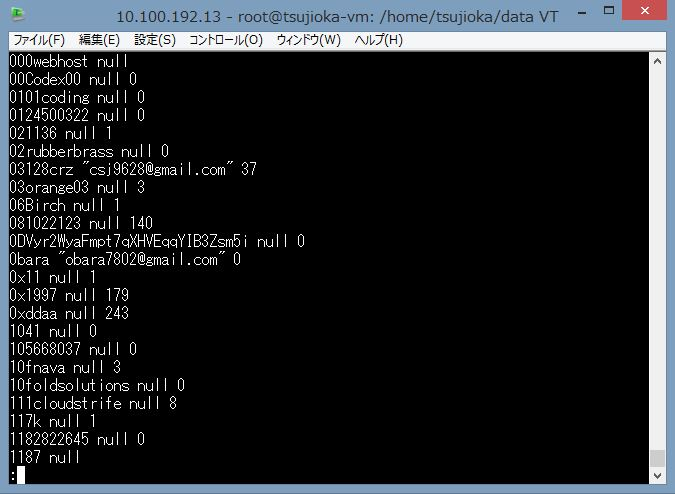
\includegraphics[width=12cm]{hoge.JPG}
\caption{データの統合}\label{サンプル図}
\end{figure}

上の画像のようなデータを取得することができたら成功である.

\newpage

emailアドレスがnullのデータは統計に使うことができないので除外しておくといい.emailアドレスがnullのデータを除外するためには次のコマンドを実行する.

\begin{lstlisting}[basicstyle=\ttfamily\footnotesize, frame=single]
gawk  '!/null/' hoge.csv > hogehoge.csv
\end{lstlisting}

%図の挿入
\begin{figure}[htb]
\centering
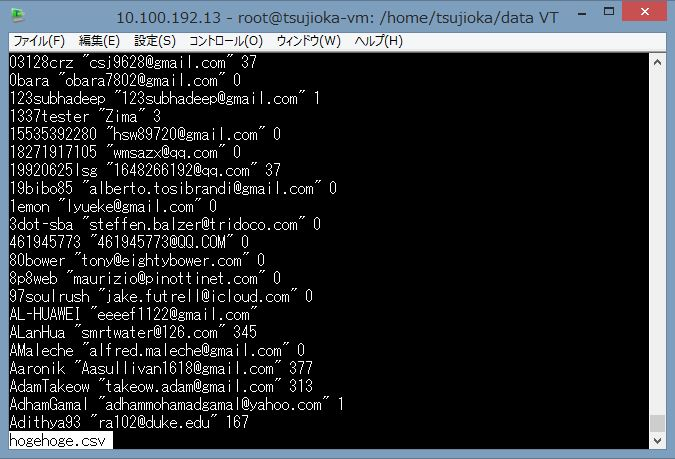
\includegraphics[width=12cm]{hogehoge.JPG}
\caption{メールアドレスNULLの除外}\label{サンプル図}
\end{figure}

上の画像のようなデータを取得することができたら成功である.


\newpage

hogehoge.csvのままでは,データとデータの区切りがダブルクオーテーションになってしまっている.ダブルクオーテーションをカンマ区切りにするためには以下のコマンドを実行する.



%図の挿入
\begin{figure}[htb]
\centering
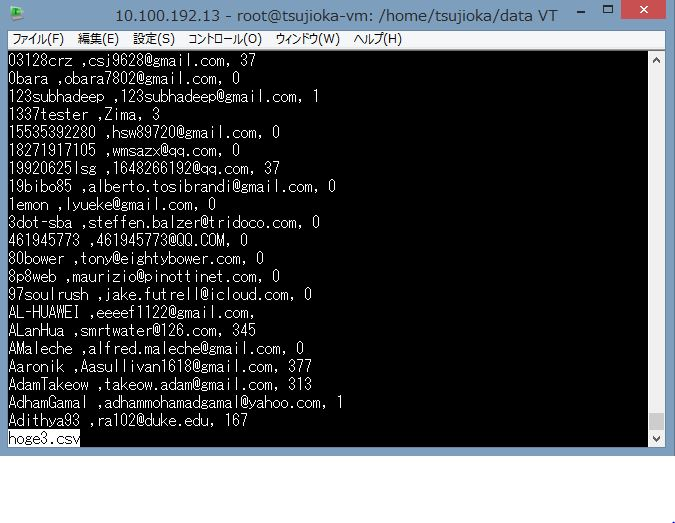
\includegraphics[width=12cm]{hoge3.JPG}
\caption{カンマ区切りへ}\label{サンプル図}
\end{figure}
上の画像のようなデータを取得することができたら成功である.
ここまででデータの取得,統合は終了である.

\newpage

\section{データの移動}
統合し終わったデータで統計を取るため仮想環境からローカルへデータの移動を行う.ファイルを移動するためteratermのSSH SCP機能を使用する.
まずは左上のファイルタブをクリックする.

%図の挿入
\begin{figure}[htb]
\centering
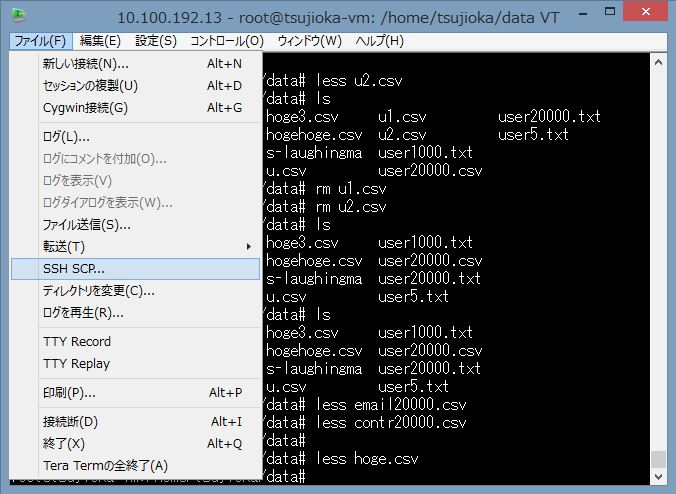
\includegraphics[width=14cm]{sshscp.JPG}
\caption{SSH SCP}\label{サンプル図}
\end{figure}

\newpage

Fromと書いてある横にあるテキストボックスに移動したいファイルを記入する.

%図の挿入
\begin{figure}[htb]
\centering
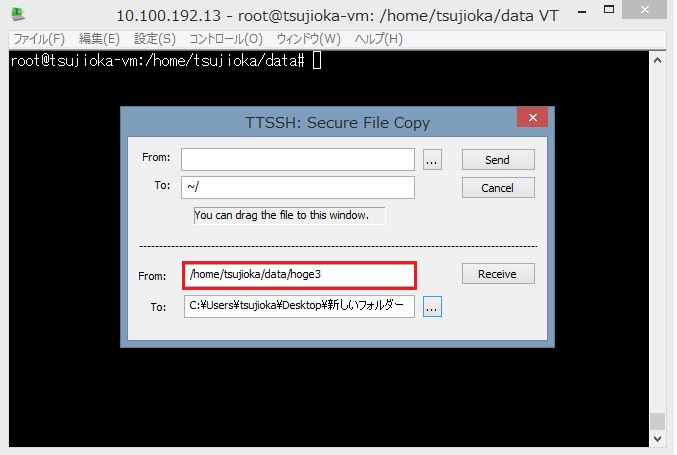
\includegraphics[width=14cm]{sshscp2.JPG}
\caption{データの選択}\label{サンプル図}
\end{figure}

\newpage

移動したいファイルを記入したテキストボックスの下にある「…」ボタンを押す.

%図の挿入
\begin{figure}[htb]
\centering
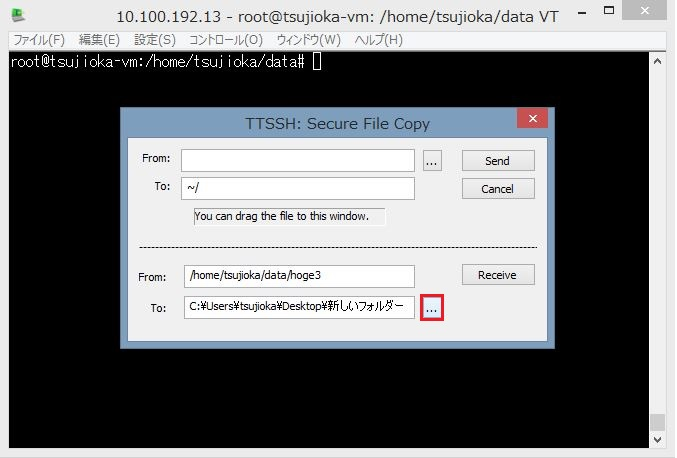
\includegraphics[width=14cm]{sshscp3.JPG}
\caption{移動場所の選択}\label{サンプル図}
\end{figure}

\newpage

フォルダーの参照というウィンドウが表示されたら,ファイルを移動する場所を選択する.

%図の挿入
\begin{figure}[htb]
\centering
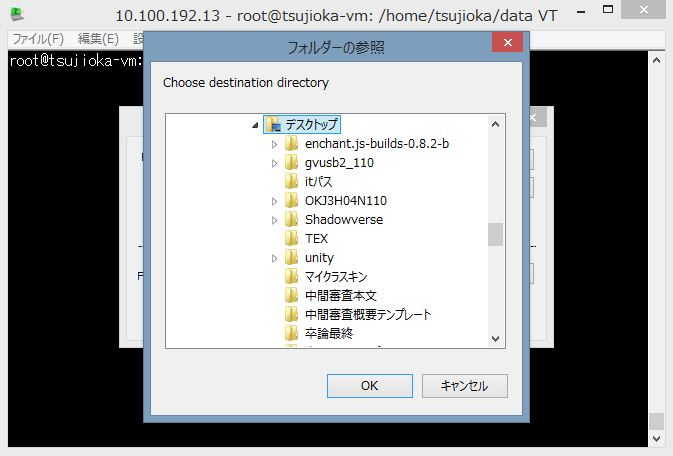
\includegraphics[width=14cm]{sshscp4.JPG}
\caption{移動場所の選択2}\label{サンプル図}
\end{figure}

\newpage

設定が完了したら右側にあるRecieveボタンを押す.

%図の挿入
\begin{figure}[htb]
\centering
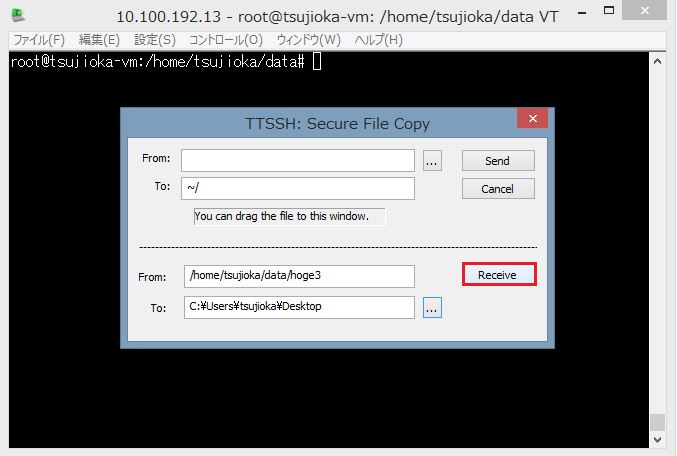
\includegraphics[width=14cm]{sshscp5.JPG}
\caption{データの移動}\label{サンプル図}
\end{figure}

選択した場所にhoge3.csvというファイルが移動していたら完了である.

\newpage

\section{統計}
hoge3.csvをxlsx形式に変換し表示してみると以下の画像のような結果が取れた.なお,取得できたデータの件数が多かったため一部抜粋して載せている.


%図の挿入
\begin{figure}[htb]
\centering
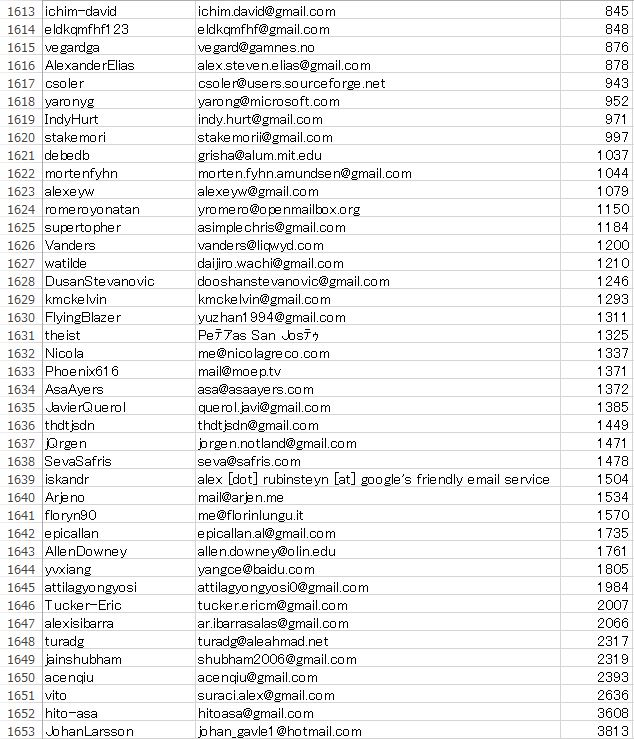
\includegraphics[width=12cm]{data2.JPG}
\caption{取得したデータの一部}\label{サンプル図}
\end{figure}

\newpage

集めたデータの中からGmailアドレスを公開しており,contributionが300以上のユーザをGoogle+で検索した.
  \begin{figure}[htb]
\centering 
\includegraphics[height=8.5cm,width=13cm]{google+.JPG}
\caption{トップ画面}
\end{figure}

上の画像がGoogle+のトップページである.ページの上部にある検索テキストボックスにGmai;アドレスを入力することでそのユーザのプロフィールを閲覧することができる.


\newpage
 
このページでフォロワー数がわかる.基本情報をクリックすることでそのユーザが公開している性別や職業などの情報を見ることができる.

\begin{figure}[htb]
\centering 
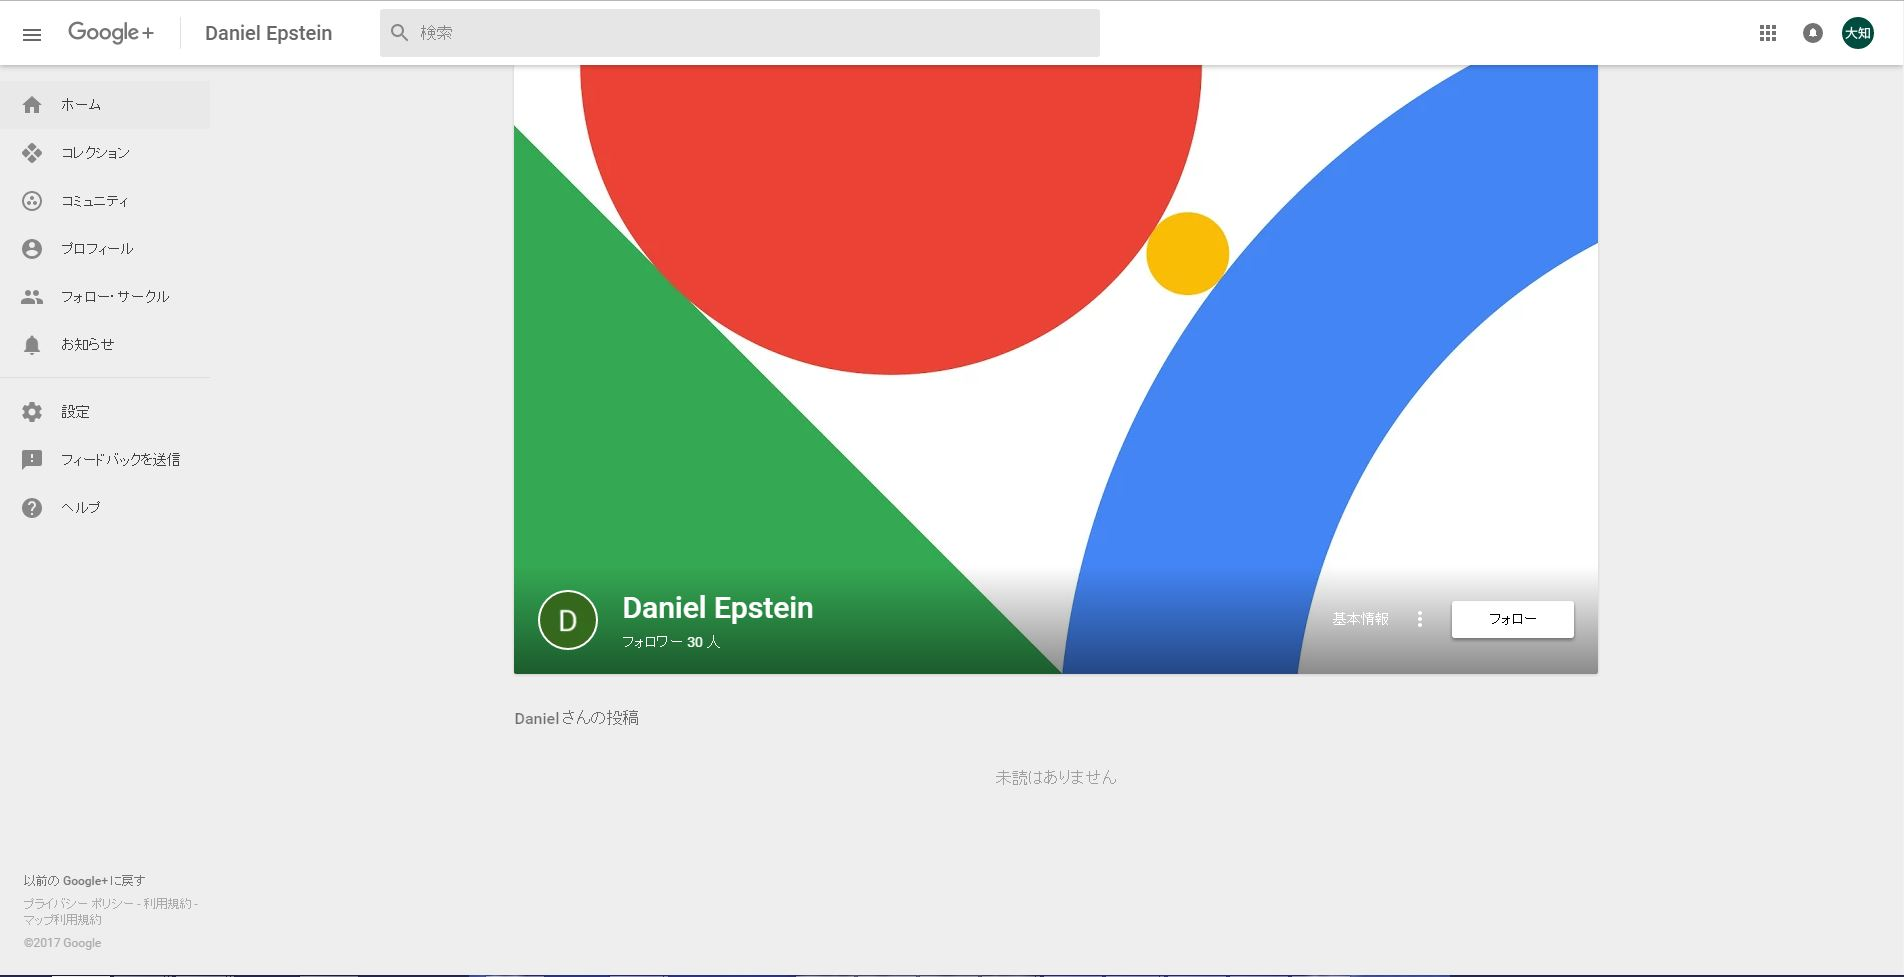
\includegraphics[height=8cm,width=13cm]{google+2.JPG}
\caption{プロフィール}
\end{figure}

\begin{figure}[htb]
\centering 
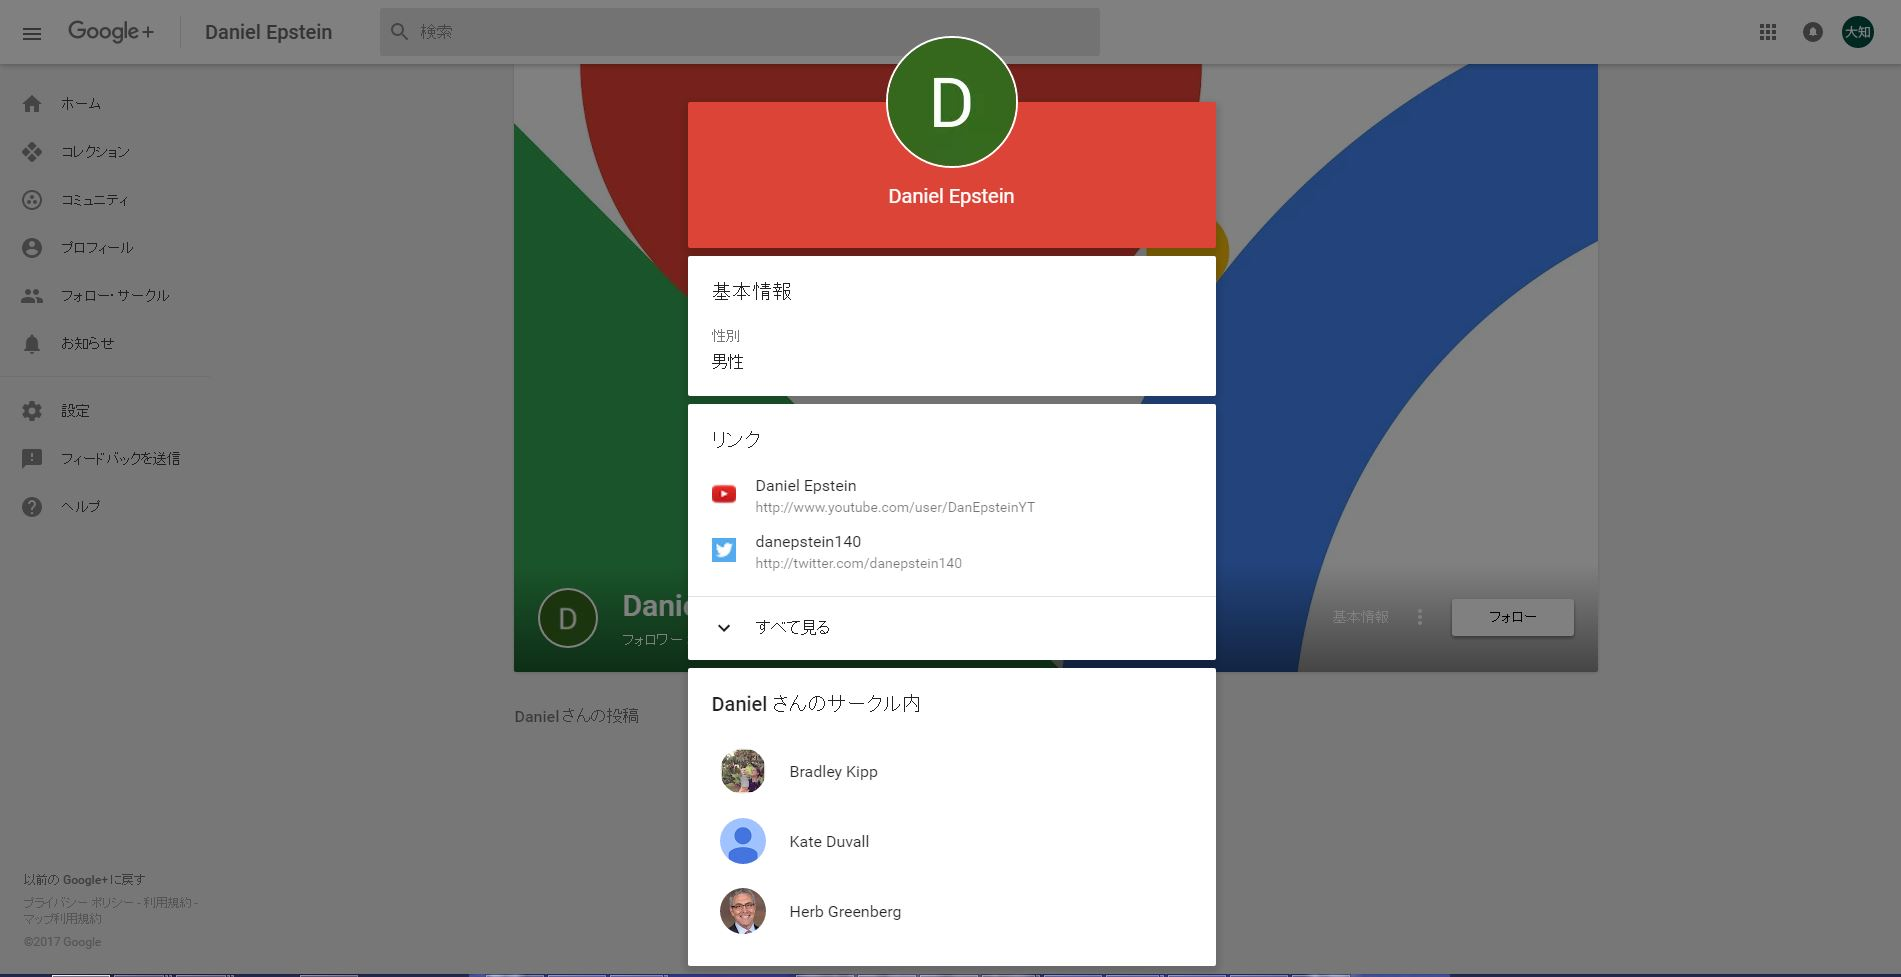
\includegraphics[height=8cm,width=13cm]{kihonn.JPG}
\caption{基本情報}
\end{figure}

\newpage

Gmailアドレスを公開しているユーザのGoogle+におけるフォロワー数を手動で集めた結果以下のようなデータが取れた.

\begin{figure}[htb]
\centering 
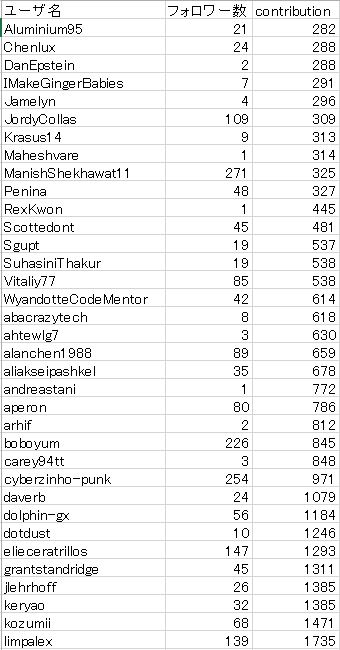
\includegraphics[height=15cm,width=9cm]{datata.JPG}
\caption{データのまとめ}
\end{figure}
手動でやった関係によりデータは35件しかとることができなかった.

\newpage

\section{回帰分析}
GitHubにおけるcontribution数とGoogle+におけるフォロワー数の相関を図るため回帰分析を行う.
\subsection{回帰分析を行うための準備作業}

まずはexcelで回帰分析を行える環境を整える必要がある.
「ファイル」→「オプション」→「アドイン」を選択すると以下の画面に遷移する.

%図の挿入
\begin{figure}[htb]
\centering
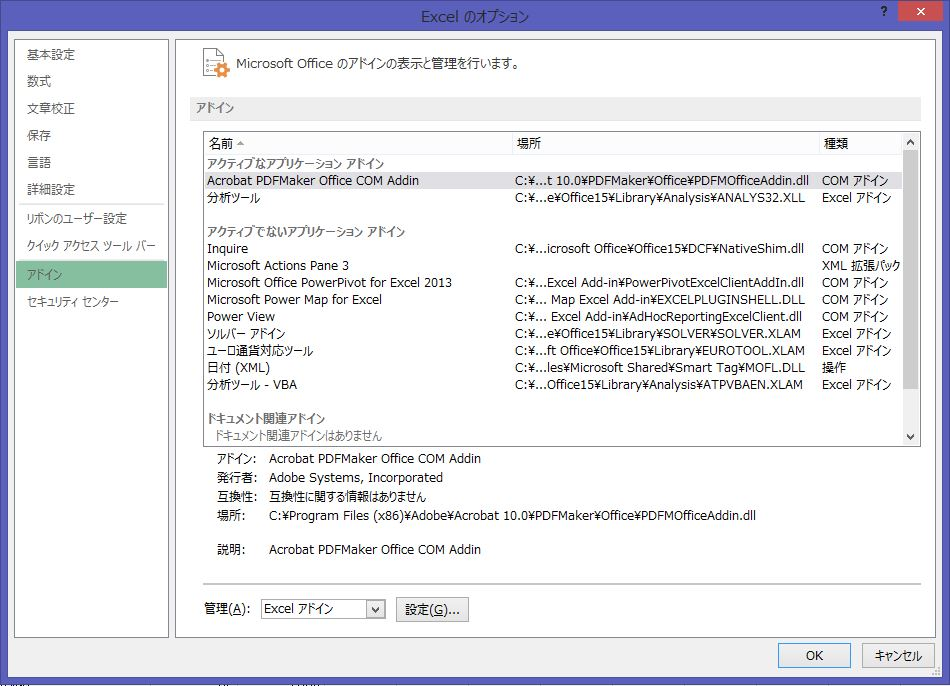
\includegraphics[width=12cm]{adoin.JPG}
\caption{回帰分析の準備}\label{サンプル図}
\end{figure}

画面の下にある「設定」ボタンをクリックすると下のような画面が表示される.
%図の挿入
\begin{figure}[htb]
\centering
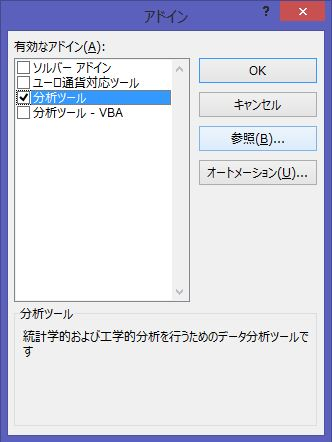
\includegraphics[height=12cm,width=9cm]{bunnseki.JPG}
\caption{回帰分析の準備2}\label{サンプル図}
\end{figure}
ここで「分析ツール」にチェックを入れて「OK」を押す.

\newpage

ここまでの準備作業を行うと「データ」のタブの一番右に「データ分析」のタブが追加されていることがわかる.
%図の挿入
\begin{figure}[htb]
\centering
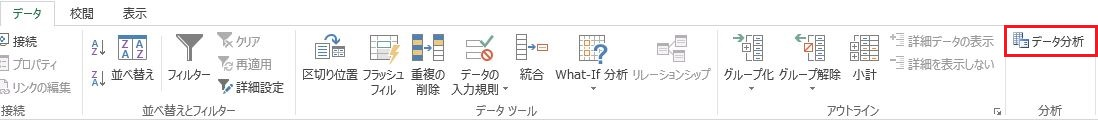
\includegraphics[height=2cm,width=15cm]{seikou.JPG}
\caption{回帰分析の準備3}\label{サンプル図}
\end{figure}
ここまでで準備作業は完了である.

\newpage

\section{回帰分析の実施}

Y軸の範囲をにフォロワー数の値,X軸の範囲をにcontributions数の値を入力し「OK」を押す. 

%図の挿入
\begin{figure}[htb]
\centering
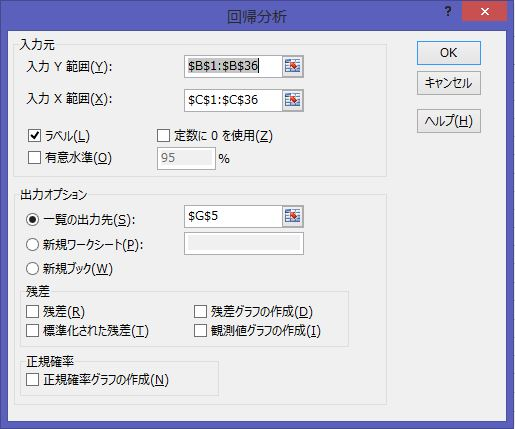
\includegraphics[width=12cm]{kaikiki.JPG}
\caption{回帰分析の実施}\label{サンプル図}
\end{figure}
結果は次章に記載する.

\newpage

\section{散布図の作成}

%図の挿入
\begin{figure}[htb]
\centering
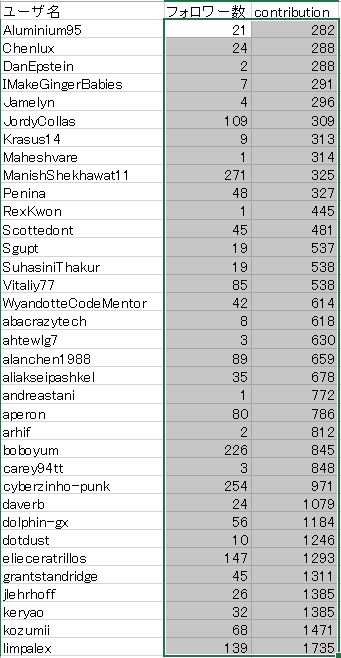
\includegraphics[height=14cm,width=8cm]{sanpu2.JPG}
\caption{データの選択}\label{サンプル図}
\end{figure}
上の画像のようにフォロワー数とcontribution数のデータを選択する.

\newpage

%図の挿入
\begin{figure}[htb]
\centering
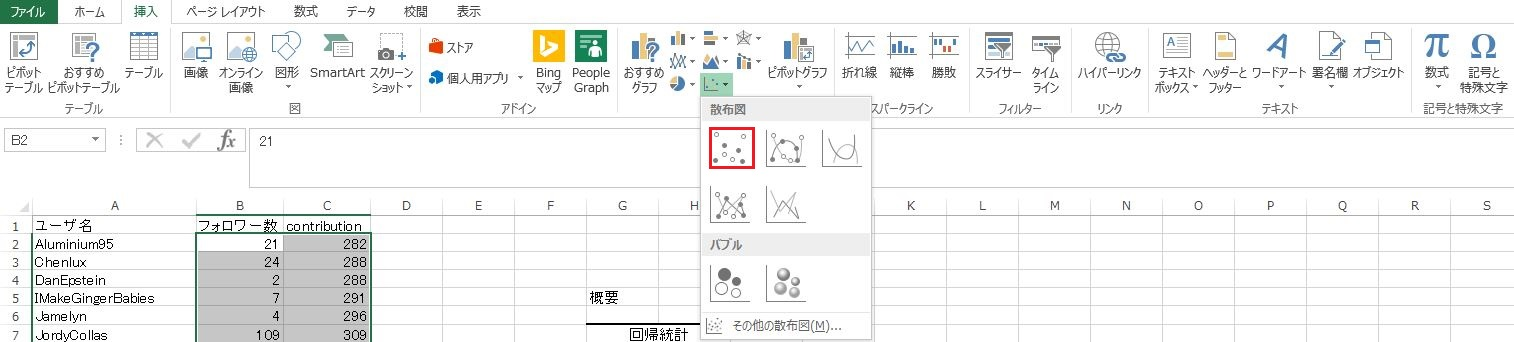
\includegraphics[height=3cm,width=15cm]{sannpu3.JPG}
\caption{グラフの選択}\label{サンプル図}
\end{figure}
選択した後,赤枠で囲ってあるグラフを選択し,グラフを作成する.
結果は次章に記載する.

\chapter{結果}

%図の挿入
\begin{figure}[htb]
\centering
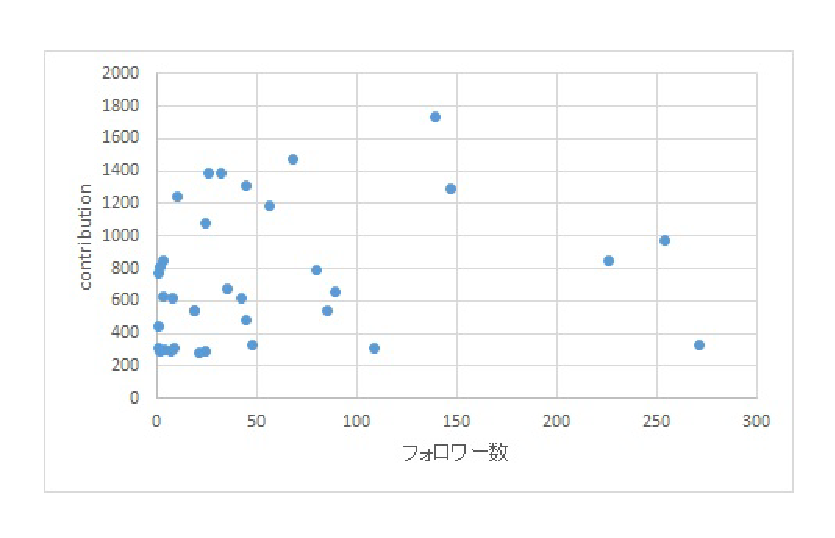
\includegraphics[width=12cm]{figure.pdf}
\caption{contributionとフォロワー数に関する散布図}\label{サンプル図}
\end{figure}

%図の挿入
\begin{figure}[htb]
\centering
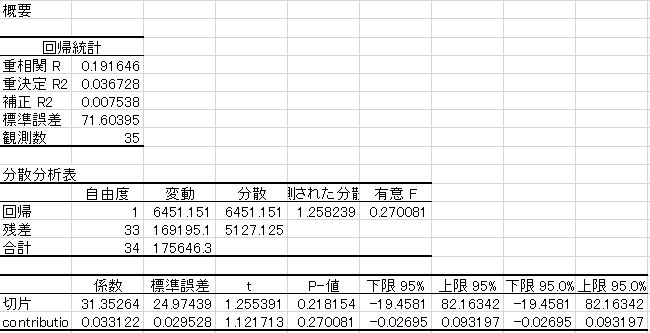
\includegraphics[width=12cm]{kaiki.JPG}
\caption{回帰分析 結果}\label{サンプル図}
\end{figure}

35件のデータを調査した結果,重相関Rの値が0.19164572316211,有意Fの値が0.27008065811877となった.この結果からGitHubにおけるcontribution数とGoogle+におけるフォロワー数に相関はないということが分かった.



\chapter{考察}

本研究を通して,活発に活動しているユーザはGoogle+におけるコミュニティが広いわけではないということが分かった.今回研究を行うためGoogle+というSNSを用いたが,現在流行しているFacebookやTwitterなどのSNSを用いることにより,今回とは違った結果が得られるのではないかと考えた.理由としてGoogle+に登録しているユーザのフォロワー数が全体的に低い傾向があるように感じた.

\chapter{結論}

本研究を通して明らかとなった相関関係などはなかった.しかし研究を進めるための過程でGHTorrent及びGoogleAPIを使用することができるようになった.今後の課題として研究を行う段階で最も流行しているSNSなどでデータを取得し,統計を取っていく必要がある.


\noindent
□□□□□□□□□■□□□□□□□□□■□□□□□□□□□■□□□□□□□□□■
□□□□□□□□□■□□□□□□□□□■□□□□□□□□□■□□□□□□□□□■
□□□□□□□□□■□□□□□□□□□■□□□□□□□□□■□□□□□□□□□■
□□□□□□□□□■□□□□□□□□□■□□□□□□□□□■□□□□□□□□□■
□□□□□□□□□■□□□□□□□□□■□□□□□□□□□■□□□□□□□□□■
□□□□□□□□□■□□□□□□□□□■□□□□□□□□□■□□□□□□□□□■
□□□□□□□□□■□□□□□□□□□■□□□□□□□□□■□□□□□□□□□■
□□□□□□□□□■□□□□□□□□□■□□□□□□□□□■□□□□□□□□□■
□□□□□□□□□■□□□□□□□□□■□□□□□□□□□■□□□□□□□□□■
□□□□□□□□□■□□□□□□□□□■□□□□□□□□□■□□□□□□□□□■
□□□□□□□□□■□□□□□□□□□■□□□□□□□□□■□□□□□□□□□■
□□□□□□□□□■□□□□□□□□□■□□□□□□□□□■□□□□□□□□□■
□□□□□□□□□■□□□□□□□□□■□□□□□□□□□■□□□□□□□□□■
□□□□□□□□□■□□□□□□□□□■□□□□□□□□□■□□□□□□□□□■
□□□□□□□□□■□□□□□□□□□■□□□□□□□□□■□□□□□□□□□■
□□□□□□□□□■□□□□□□□□□■□□□□□□□□□■□□□□□□□□□■
□□□□□□□□□■□□□□□□□□□■□□□□□□□□□■□□□□□□□□□■
□□□□□□□□□■□□□□□□□□□■□□□□□□□□□■□□□□□□□□□■
□□□□□□□□□■□□□□□□□□□■□□□□□□□□□■□□□□□□□□□■
□□□□□□□□□■□□□□□□□□□■□□□□□□□□□■□□□□□□□□□■
□□□□□□□□□■□□□□□□□□□■□□□□□□□□□■□□□□□□□□□■
□□□□□□□□□■□□□□□□□□□■□□□□□□□□□■□□□□□□□□□■
□□□□□□□□□■□□□□□□□□□■□□□□□□□□□■□□□□□□□□□■
□□□□□□□□□■□□□□□□□□□■□□□□□□□□□■□□□□□□□□□■
□□□□□□□□□■□□□□□□□□□■□□□□□□□□□■□□□□□□□□□■
□□□□□□□□□■□□□□□□□□□■□□□□□□□□□■□□□□□□□□□■
□□□□□□□□□■□□□□□□□□□■□□□□□□□□□■□□□□□□□□□■
□□□□□□□□□■□□□□□□□□□■□□□□□□□□□■□□□□□□□□□■
□□□□□□□□□■□□□□□□□□□■□□□□□□□□□■□□□□□□□□□■
□□□□□□□□□■□□□□□□□□□■□□□□□□□□□■□□□□□□□□□■
□□□□□□□□□■□□□□□□□□□■□□□□□□□□□■□□□□□□□□□■
□□□□□□□□□■□□□□□□□□□■□□□□□□□□□■□□□□□□□□□■
□□□□□□□□□■□□□□□□□□□■□□□□□□□□□■□□□□□□□□□■
□□□□□□□□□■□□□□□□□□□■□□□□□□□□□■□□□□□□□□□■
□□□□□□□□□■□□□□□□□□□■□□□□□□□□□■□□□□□□□□□■
□□□□□□□□□■□□□□□□□□□■□□□□□□□□□■□□□□□□□□□■
□□□□□□□□□■□□□□□□□□□■□□□□□□□□□■□□□□□□□□□■
□□□□□□□□□■□□□□□□□□□■□□□□□□□□□■□□□□□□□□□■
□□□□□□□□□■□□□□□□□□□■□□□□□□□□□■□□□□□□□□□■
■■■■■■■■■■■■■■■■■■■■■■■■■■■■■■■■■■■■■■■■
□□□□□□□□□■□□□□□□□□□■□□□□□□□□□■□□□□□□□□□■

\bibliographystyle{junsrt}
\bibliography{biblio}%「biblio.bib」というファイルが必要.



\end{document}
